%%%%%%%%%%%%%%%%%%%%%%%%%%%%%%%%%%%%%%%%%%%%%%%%%%%%%%%%%%%%%%%%%%%%%%%%%%%%%%%%
\section{Lecture 3: Climate variability on a timescale of thousands of years}

2 driving forces for climate variability:
\begin{itemize}
    \item Orbital forcing
    \item Tectonic forcing
\end{itemize}

\textit{Forcing} means something external driving the climate.

Ice age is a long geological interval during which there are glaciations. The
current ice age started at the beginning of the Quaternary period.

Multiple glaciations and interglacials happened in current ice age. They occur
in cycles driven by the orbital cycles.

\begin{figure}[H]
    \centering
    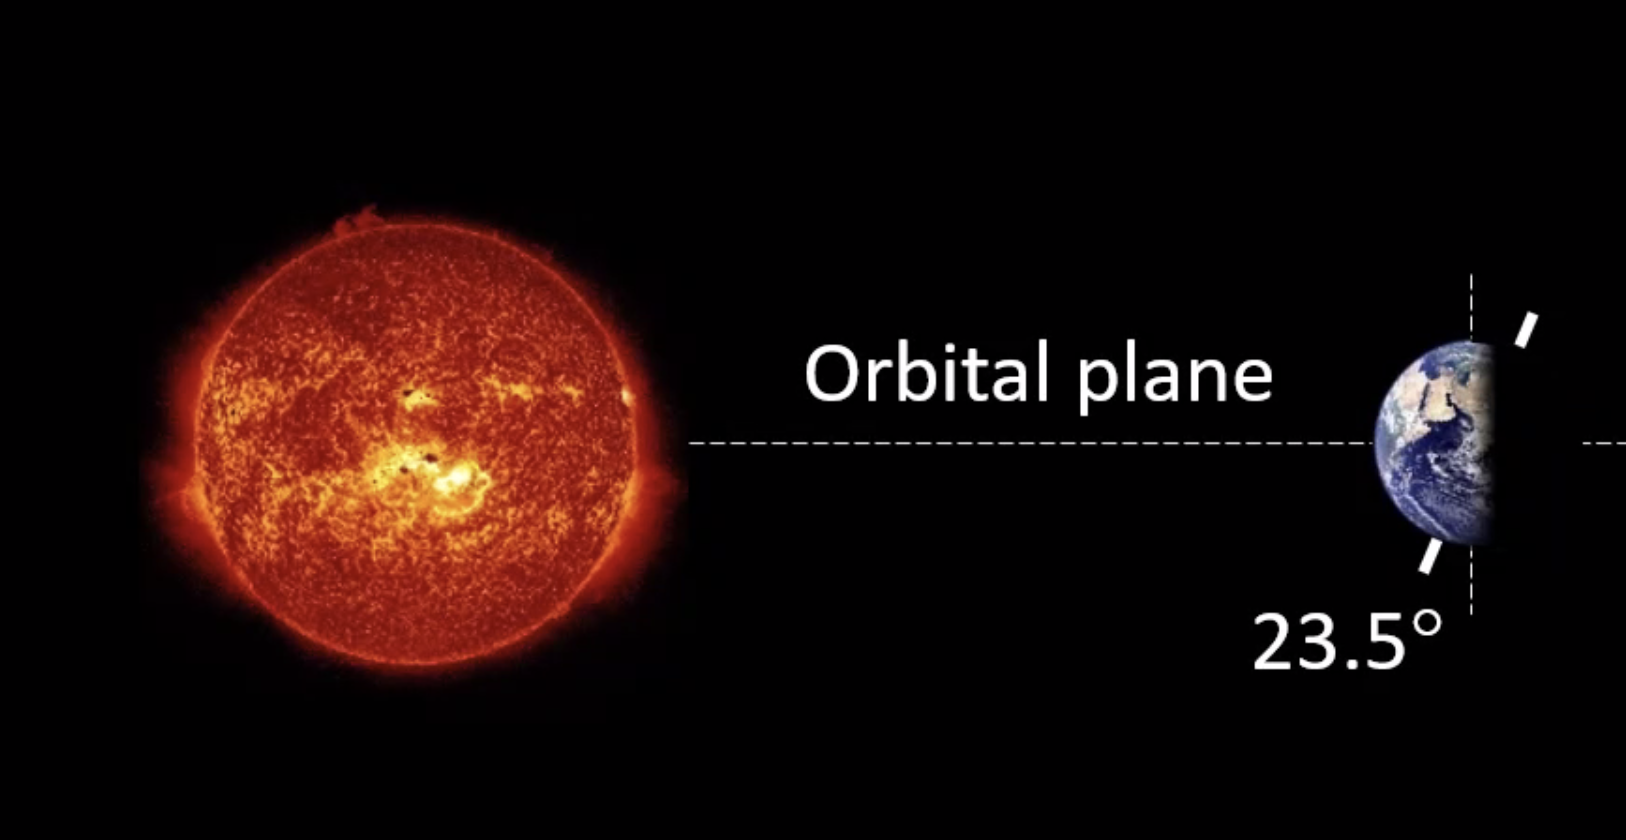
\includegraphics[width=0.5\linewidth]{content/img/axial_tilt.png}
    \caption{Current axial tilt is $23.5 \degree$}
\end{figure}

Earth's orbit is an ellipse. Sun is in one of its focal points.

\textbf{Perihelion} is when the Earth is the closest to the Sun, currently
153km (but changes depending on orbit's \textit{eccentricity}).

\textbf{Aphelion} is the furthest the Earth can be from the sun, currently
158km.

If axial tilt was $0 \degree$, there would be no seasons.

If axial tilt was $90 \degree$, there would be extreme seasonality.

%%%%%%%%%%%%%%%%%%%%%%%%%%%%%%%%%%%%%%%%%%%%%%%%%%%%%%%%%%%%%%%%%%%%%%%%%%%%%%%%
\textbf{Milankovic cycles}:

\begin{itemize}
    \item \textbf{axial tilt}: 41000 years cycle between $22.1 \degree$ and
    $24.5 \degree$
    \item \textbf{eccentricity}: 100000 and 413000 cycles, changes due to
    gravitational
    effect of other planets
    \item \textbf{precession} (wobble) of perihelion and aphelion along the
    orbit
\end{itemize}

\begin{figure}[H]
    \centering
    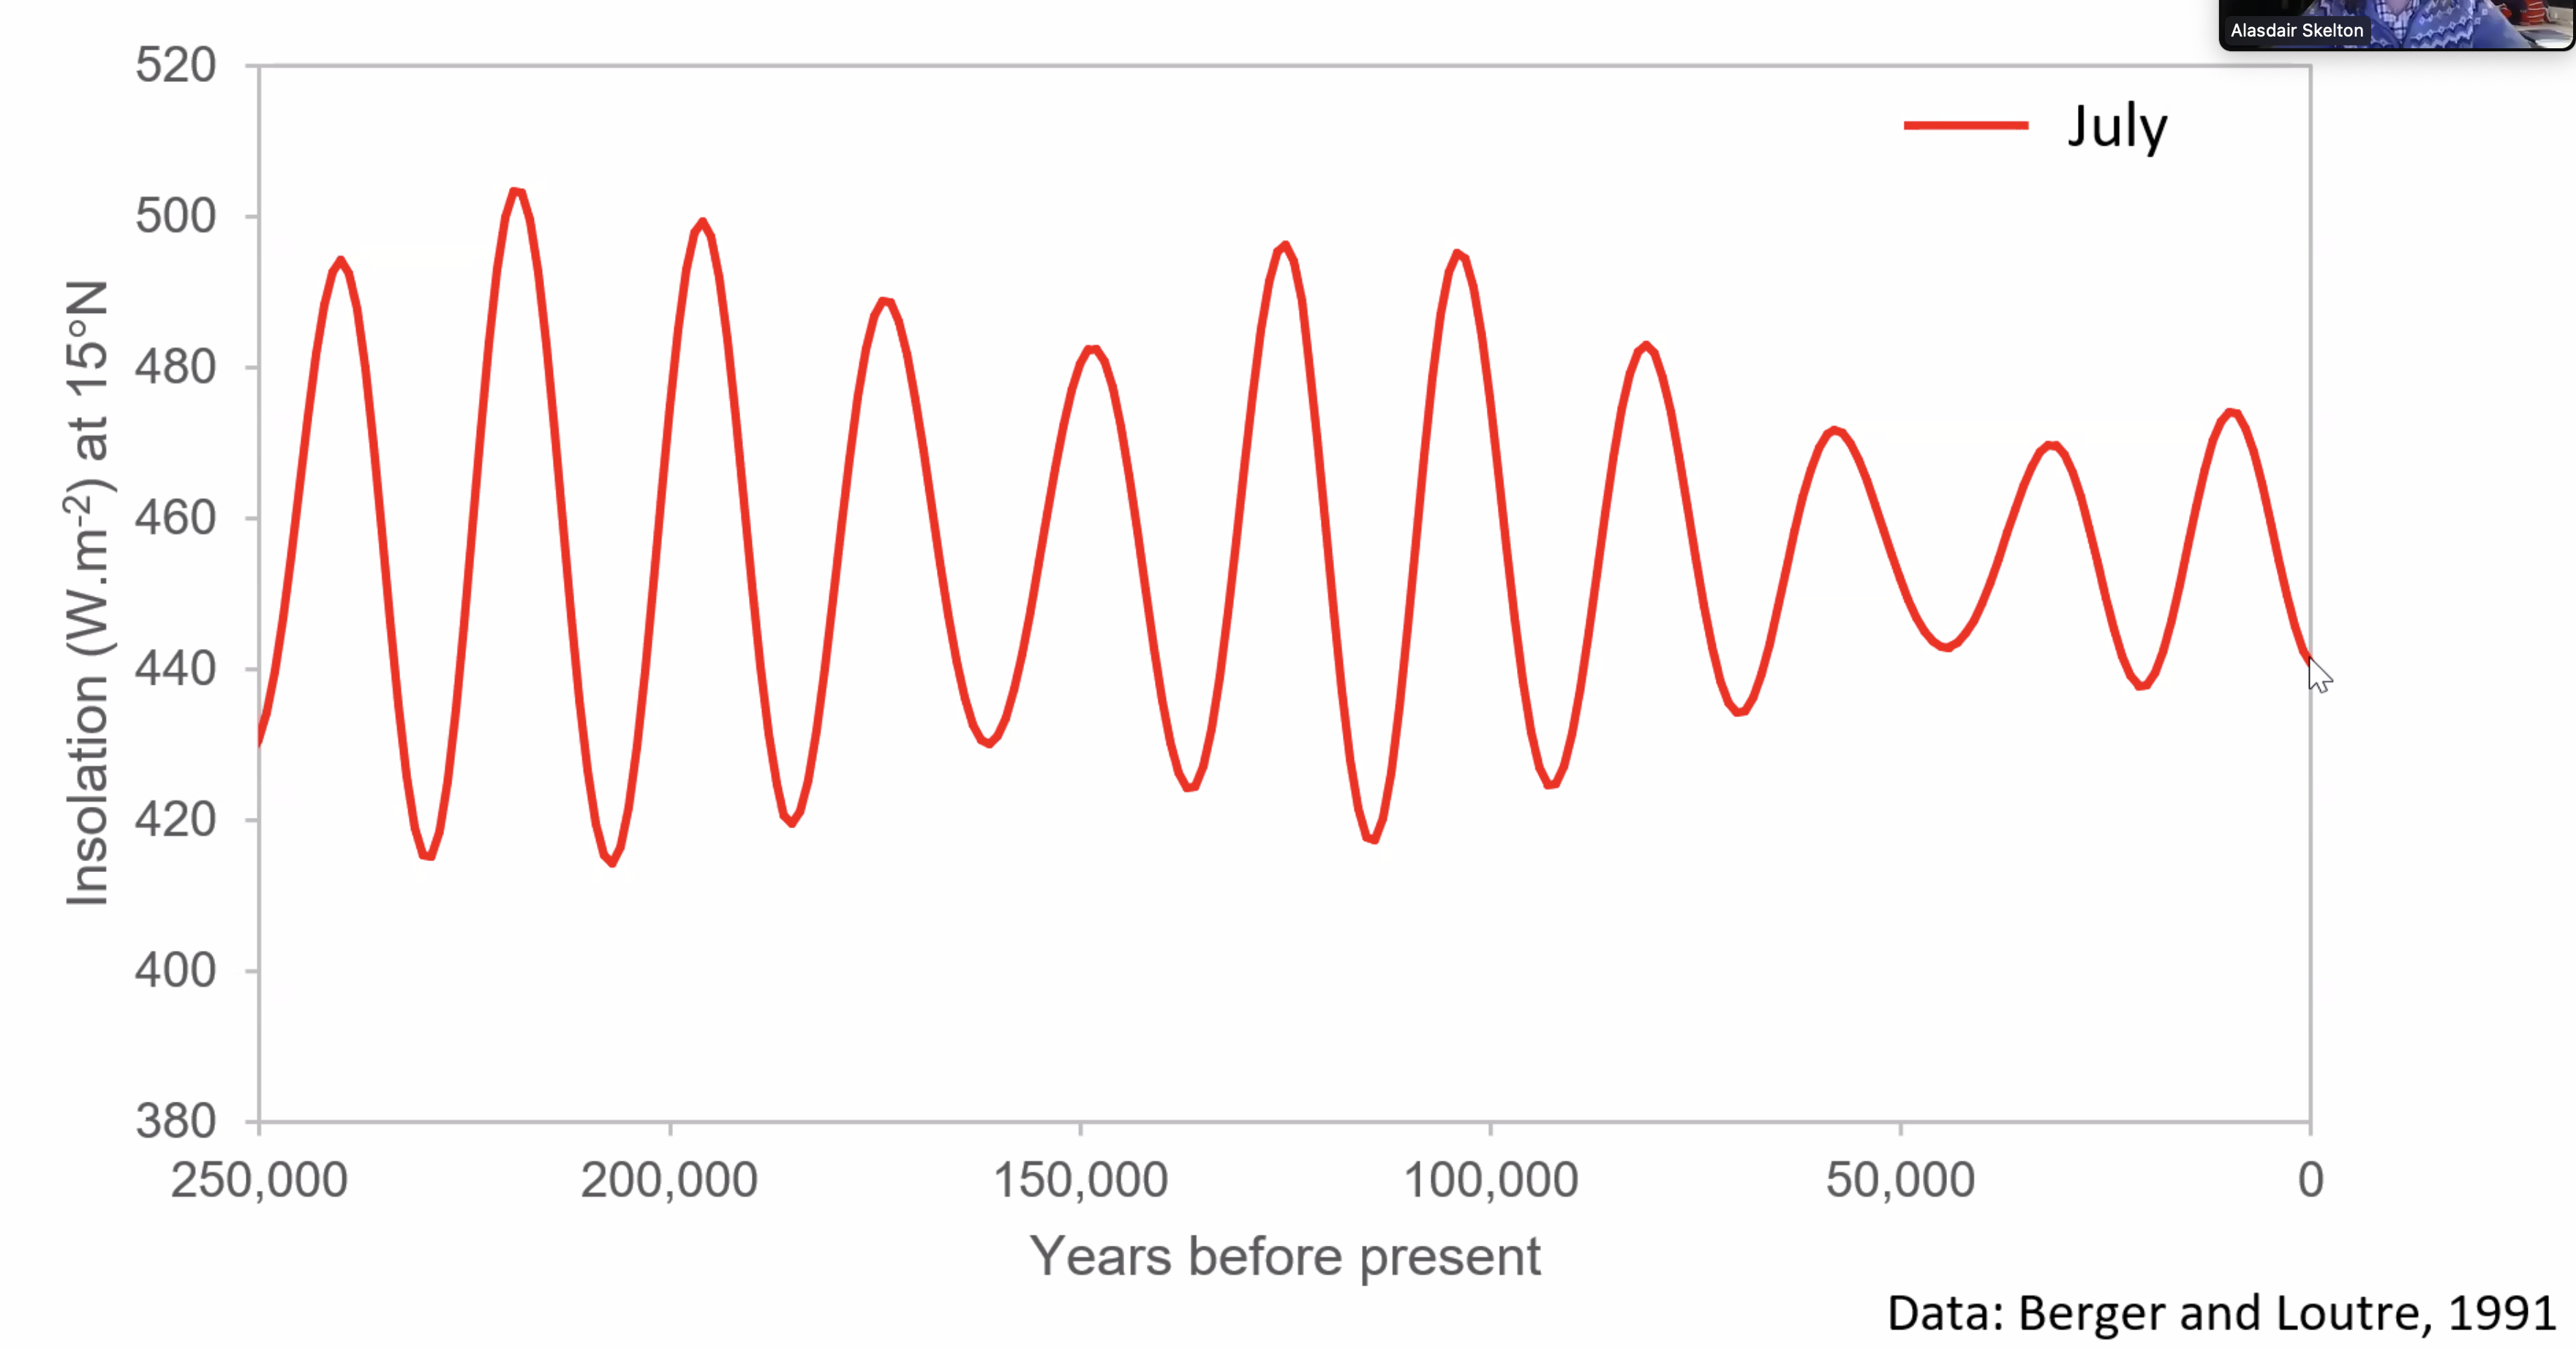
\includegraphics[width=1.0\linewidth]{content/img/insolation_in_july.png}
    \caption{Insolation in July}
\end{figure}

\begin{figure}[H]
    \centering
    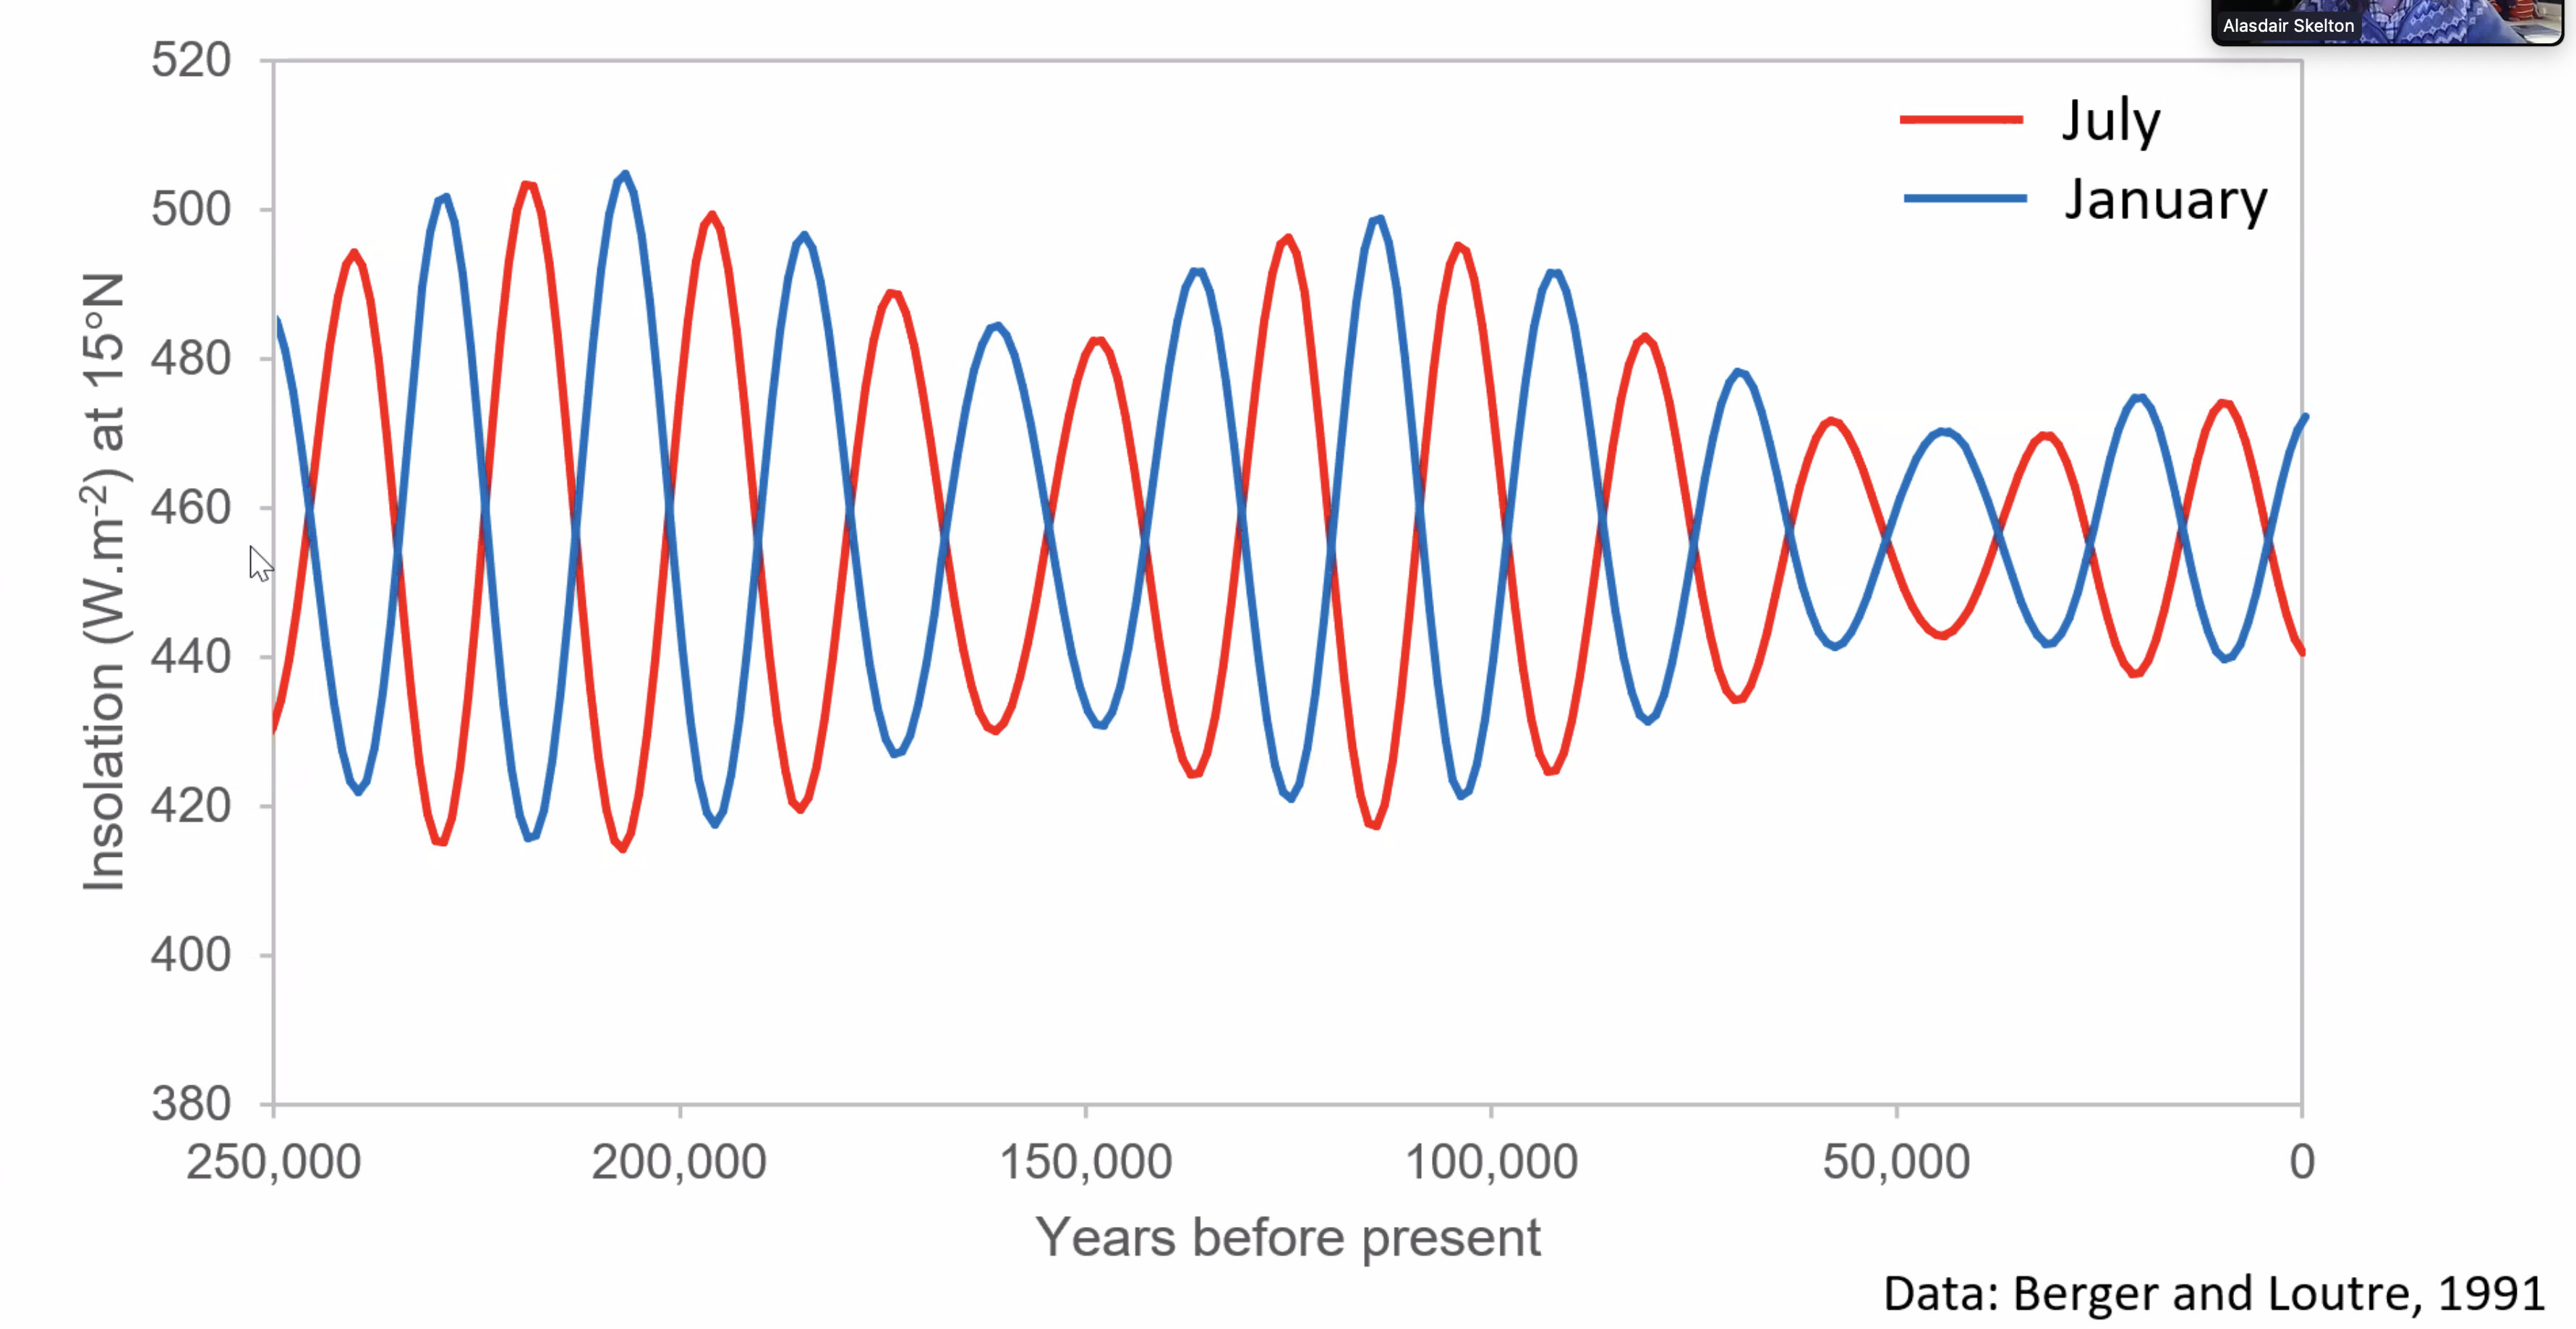
\includegraphics[width=1\linewidth]{content/img/insolation_july_january.png}
    \caption{Insolation in July and January}
\end{figure}

Milankovic cycles drive glaciations, not the other way around.

\subsection{Monsoons}

\begin{figure}[H]
    \centering
    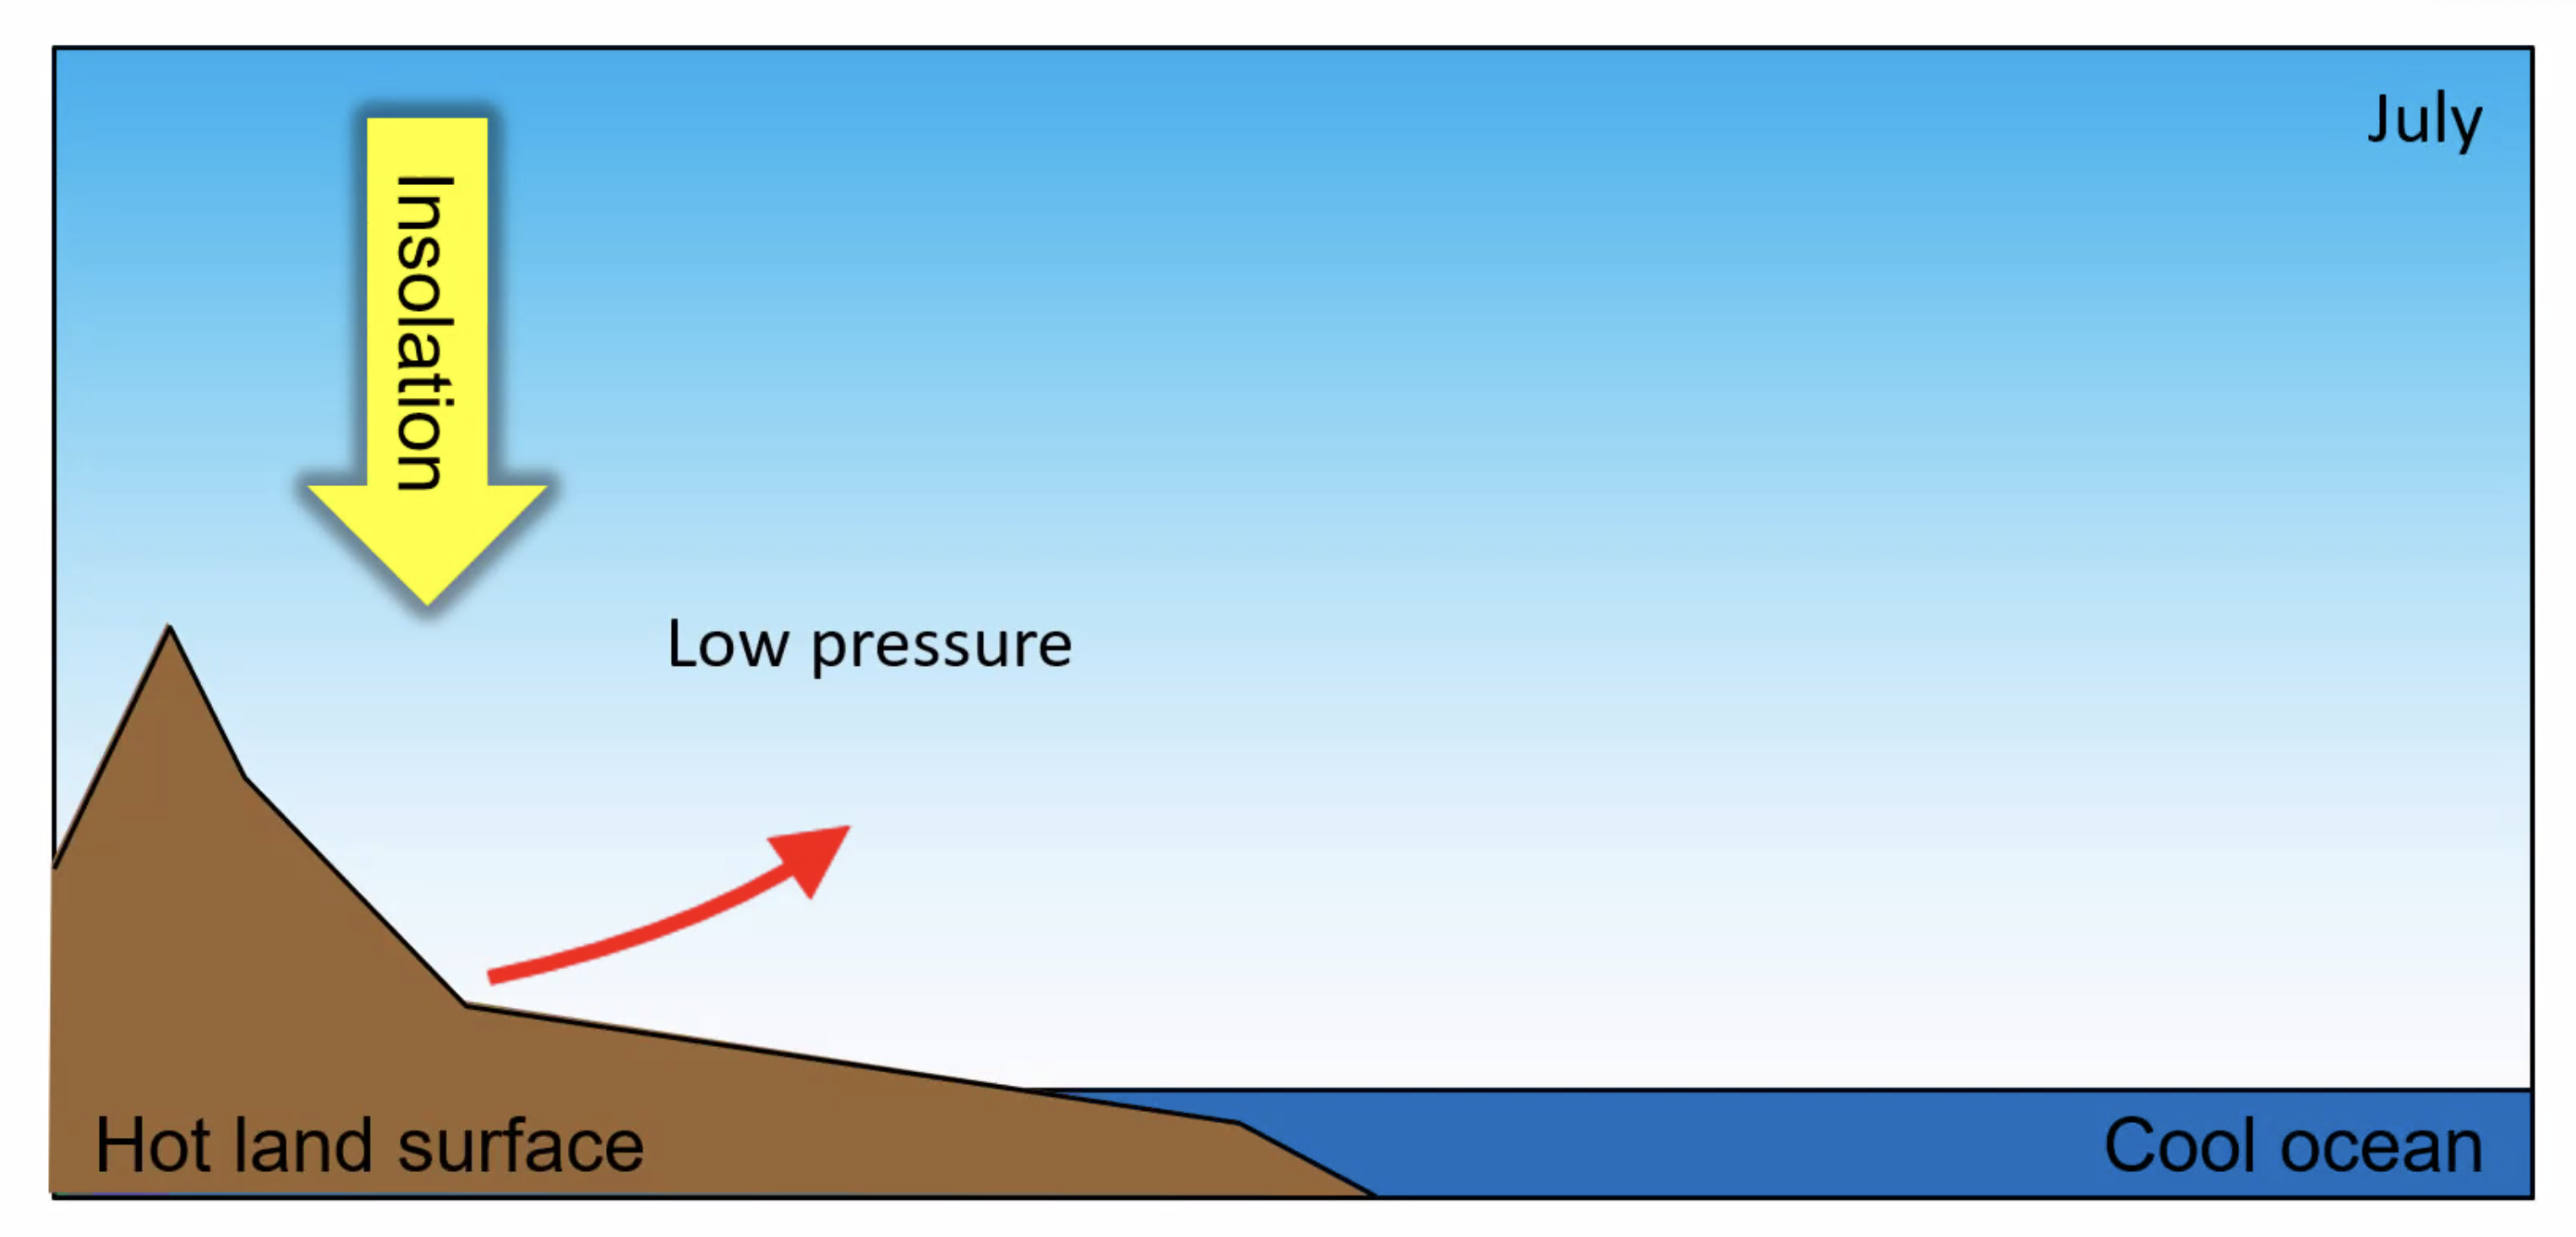
\includegraphics[width=0.5\linewidth]{content/img/monsoon_1.png}
    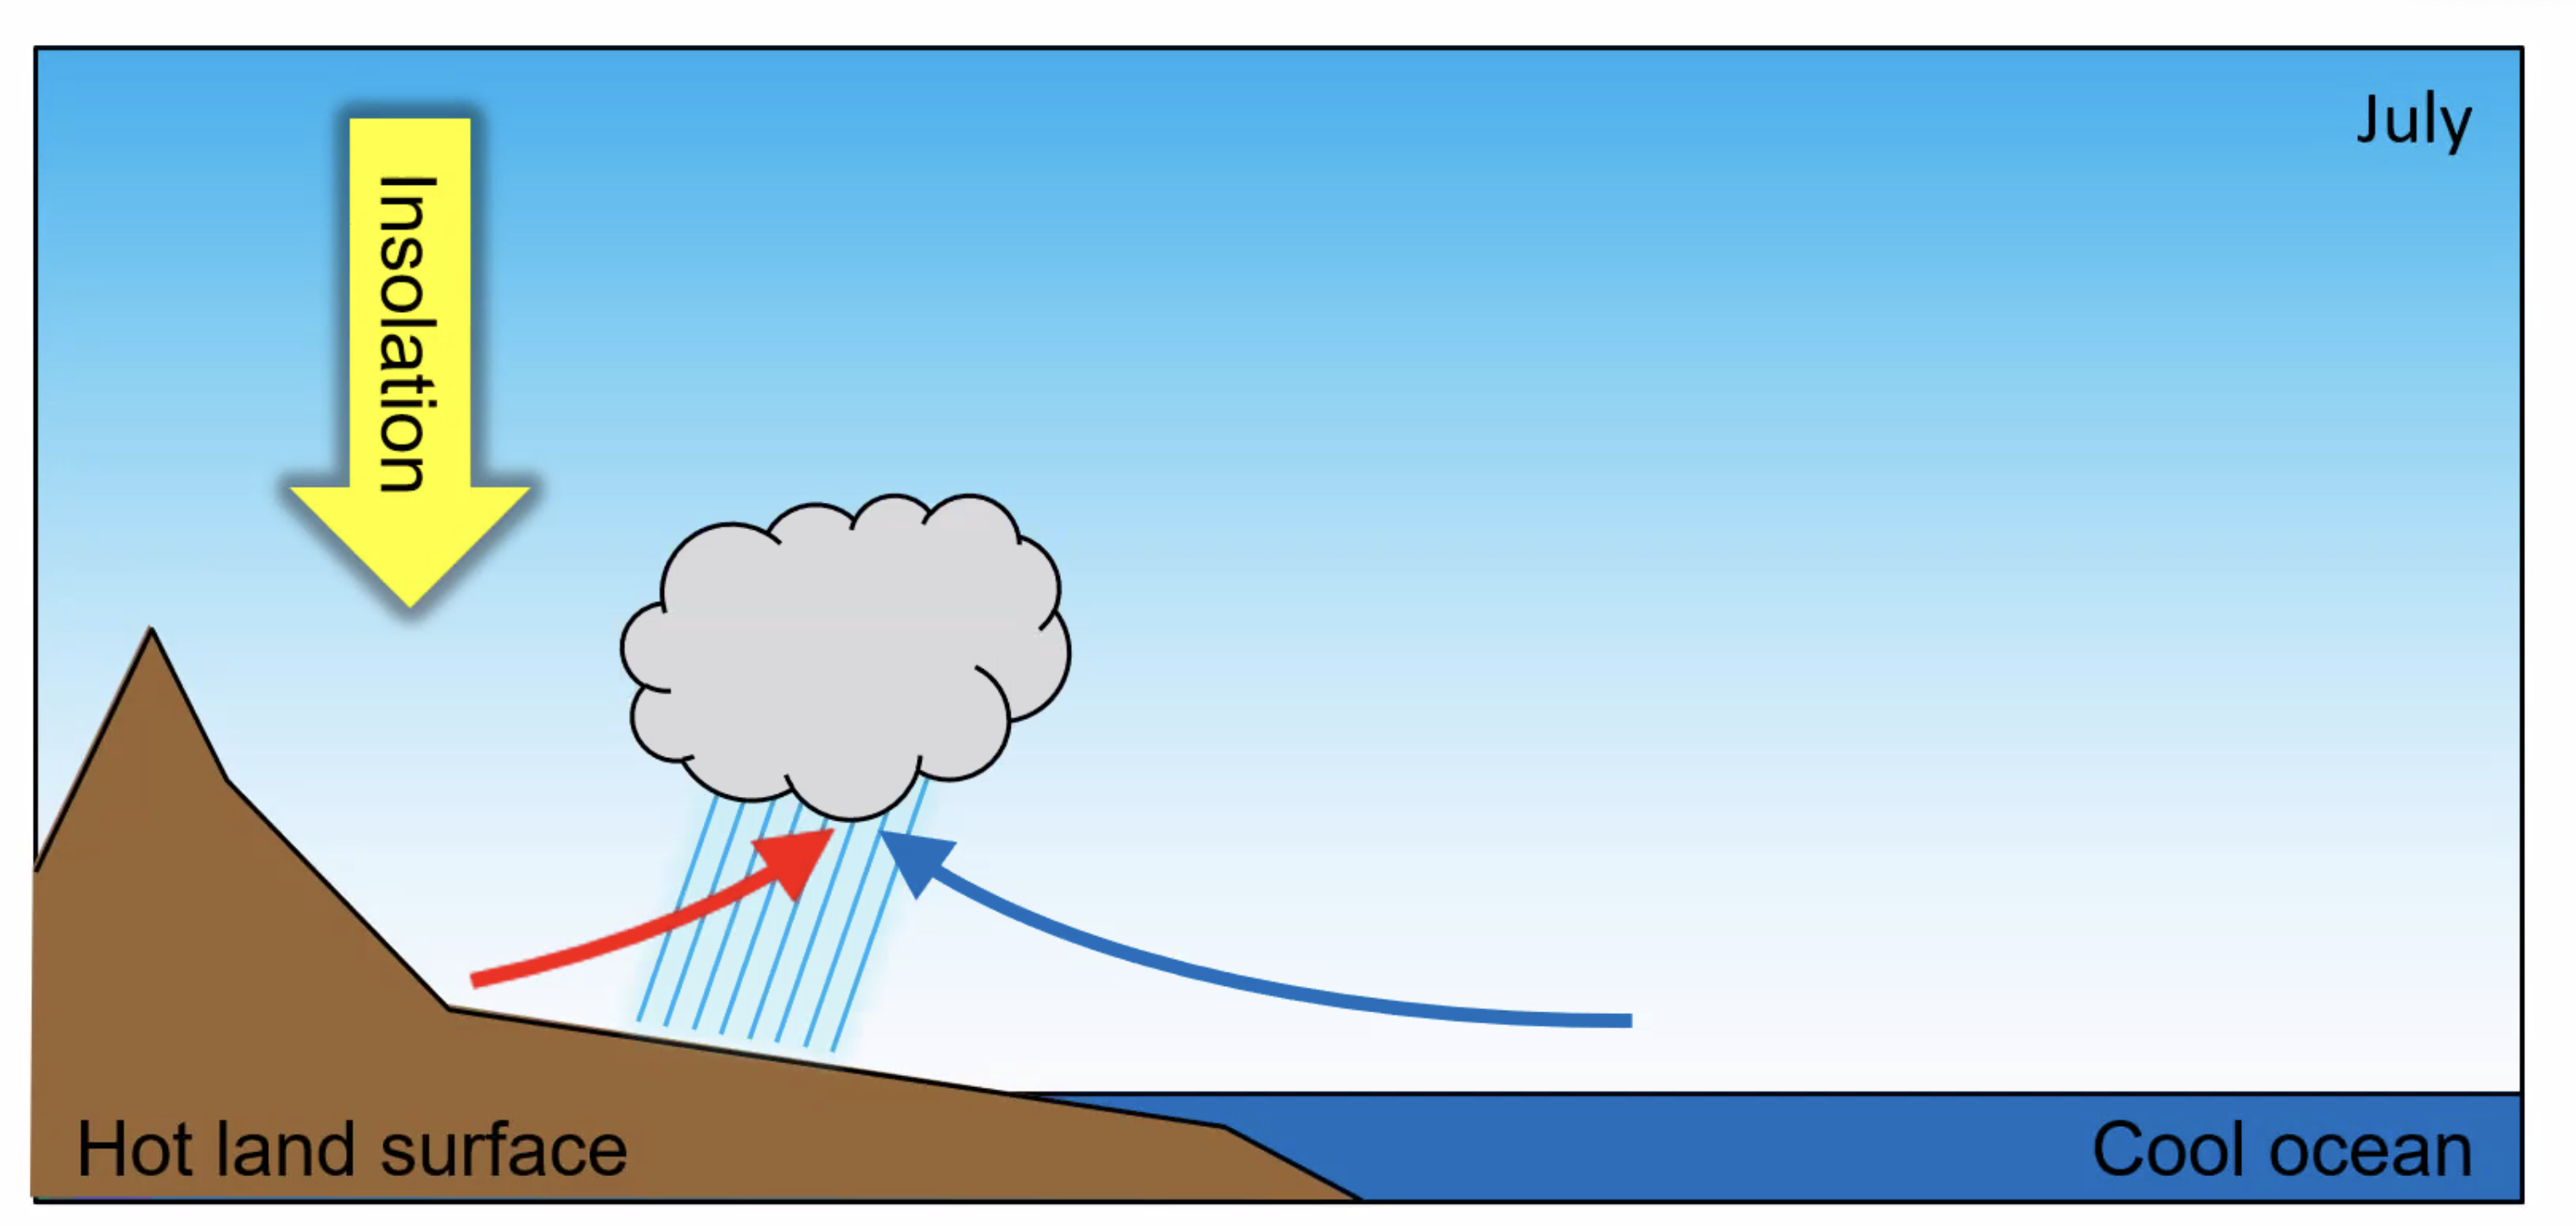
\includegraphics[width=0.5\linewidth]{content/img/monsoon_2.png}
    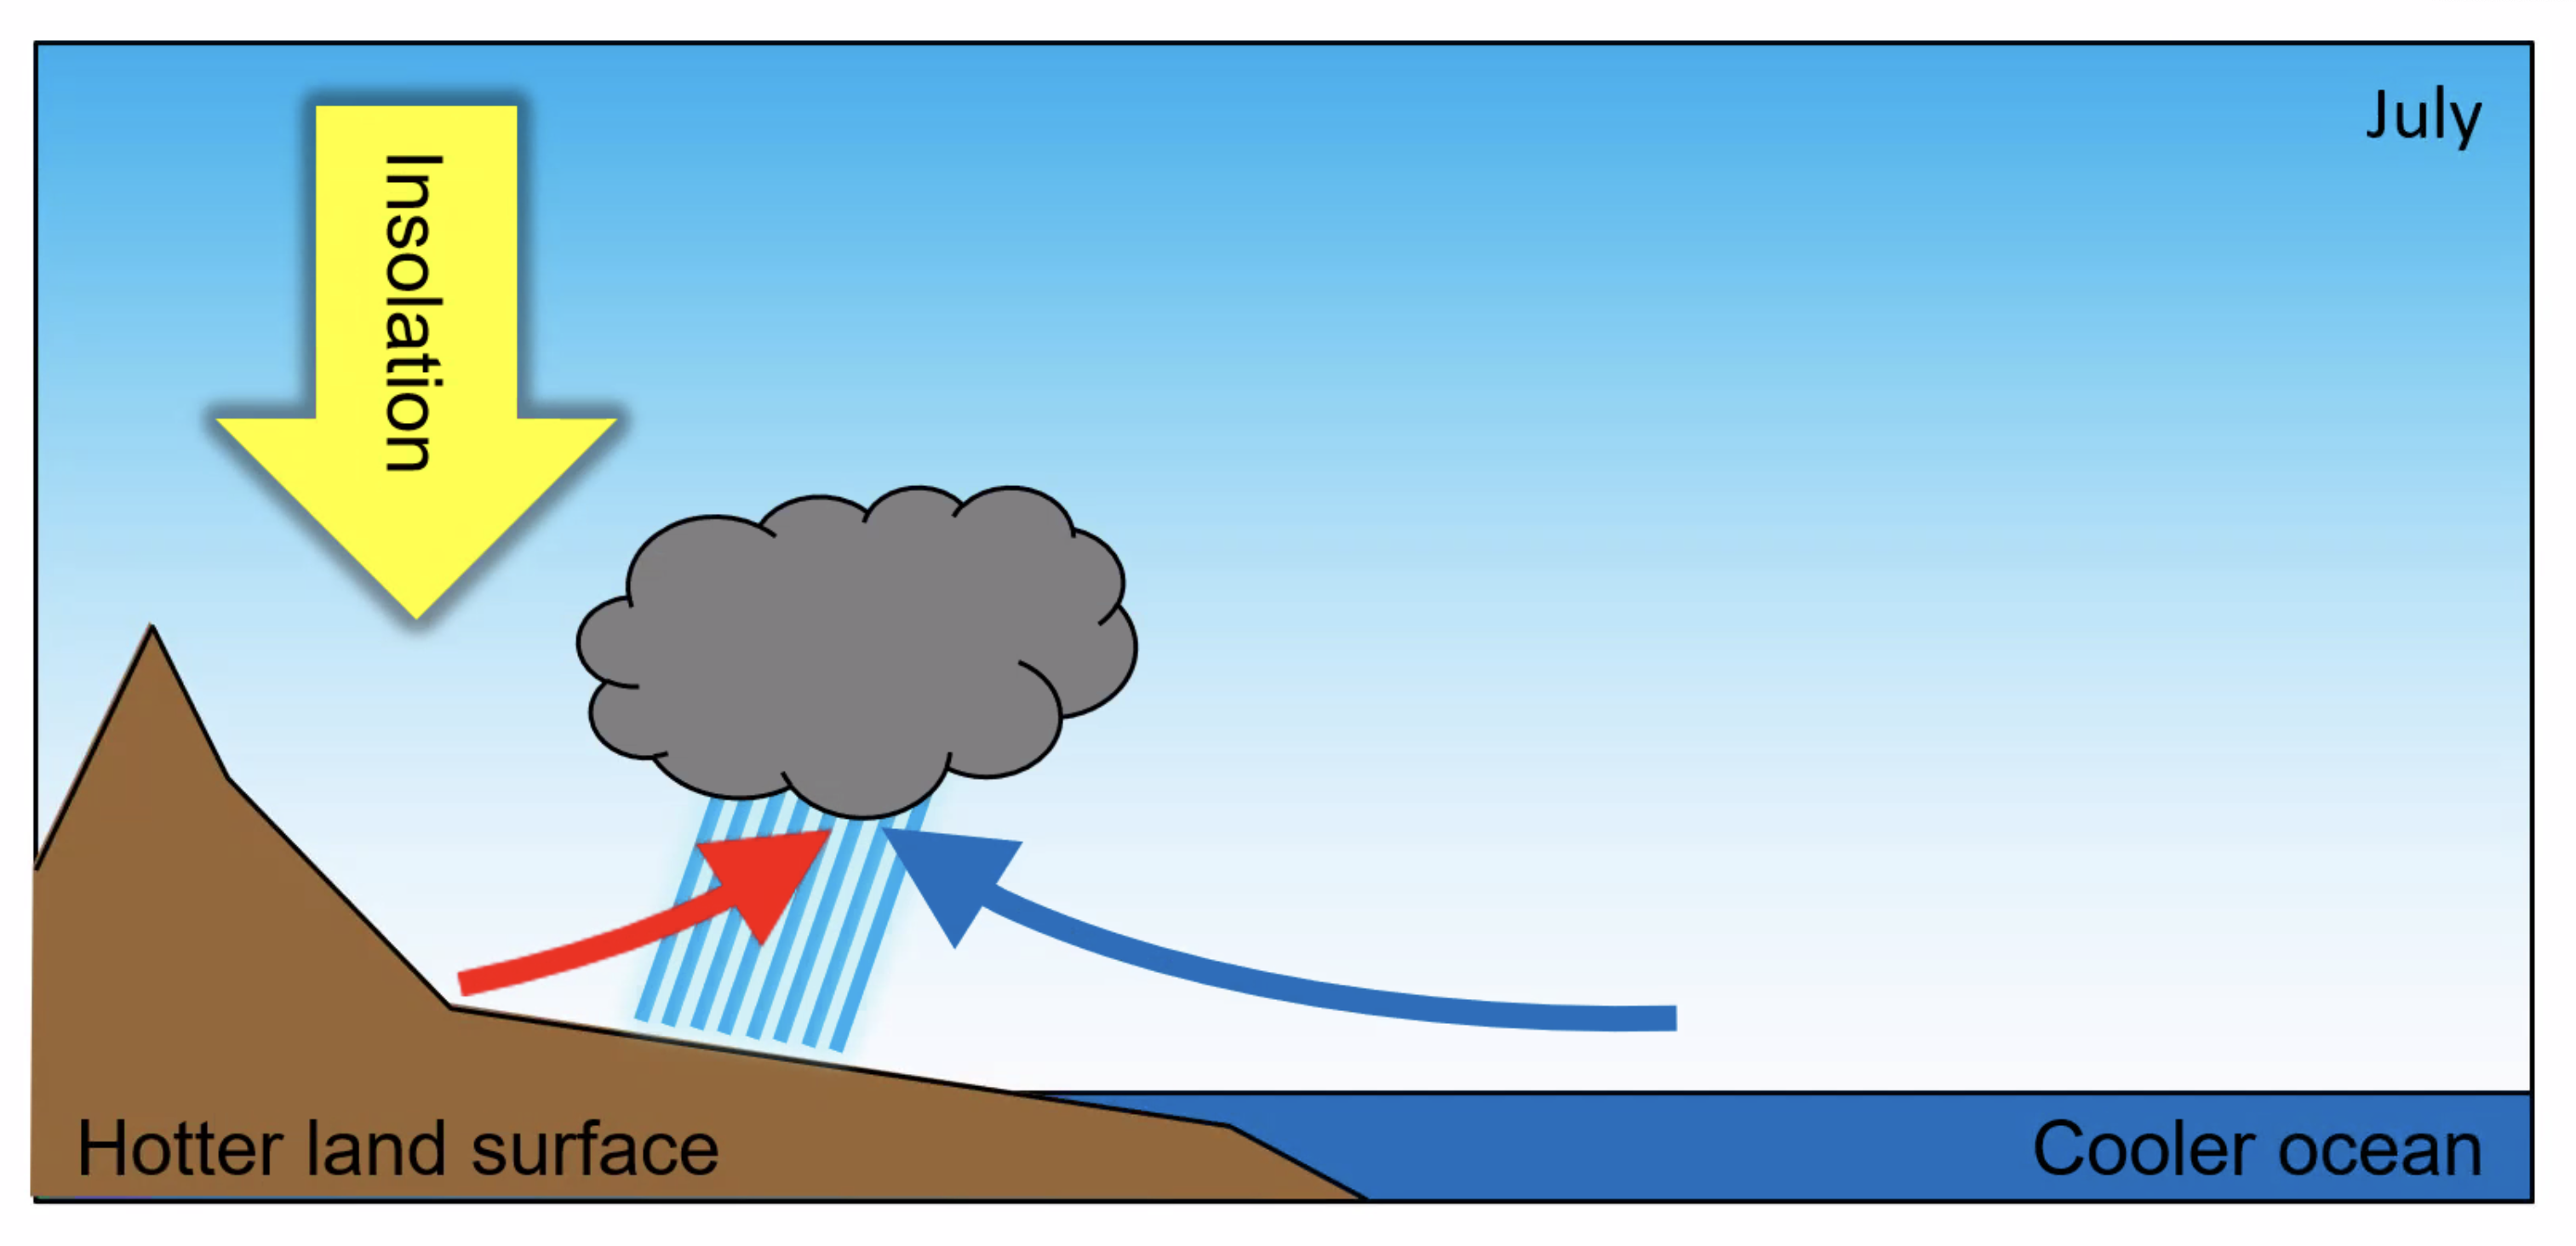
\includegraphics[width=0.5\linewidth]{content/img/monsoon_3.png}
    \caption{Summer monsoon}
\end{figure}

%%%%%%%%%%%%%%%%%%%%%%%%%%%%%%%%%%%%%%%%%%%%%%%%%%%%%%%%%%%%%%%%%%%%%%%%%%%%%%%%
\begin{figure}[H]
    \centering
    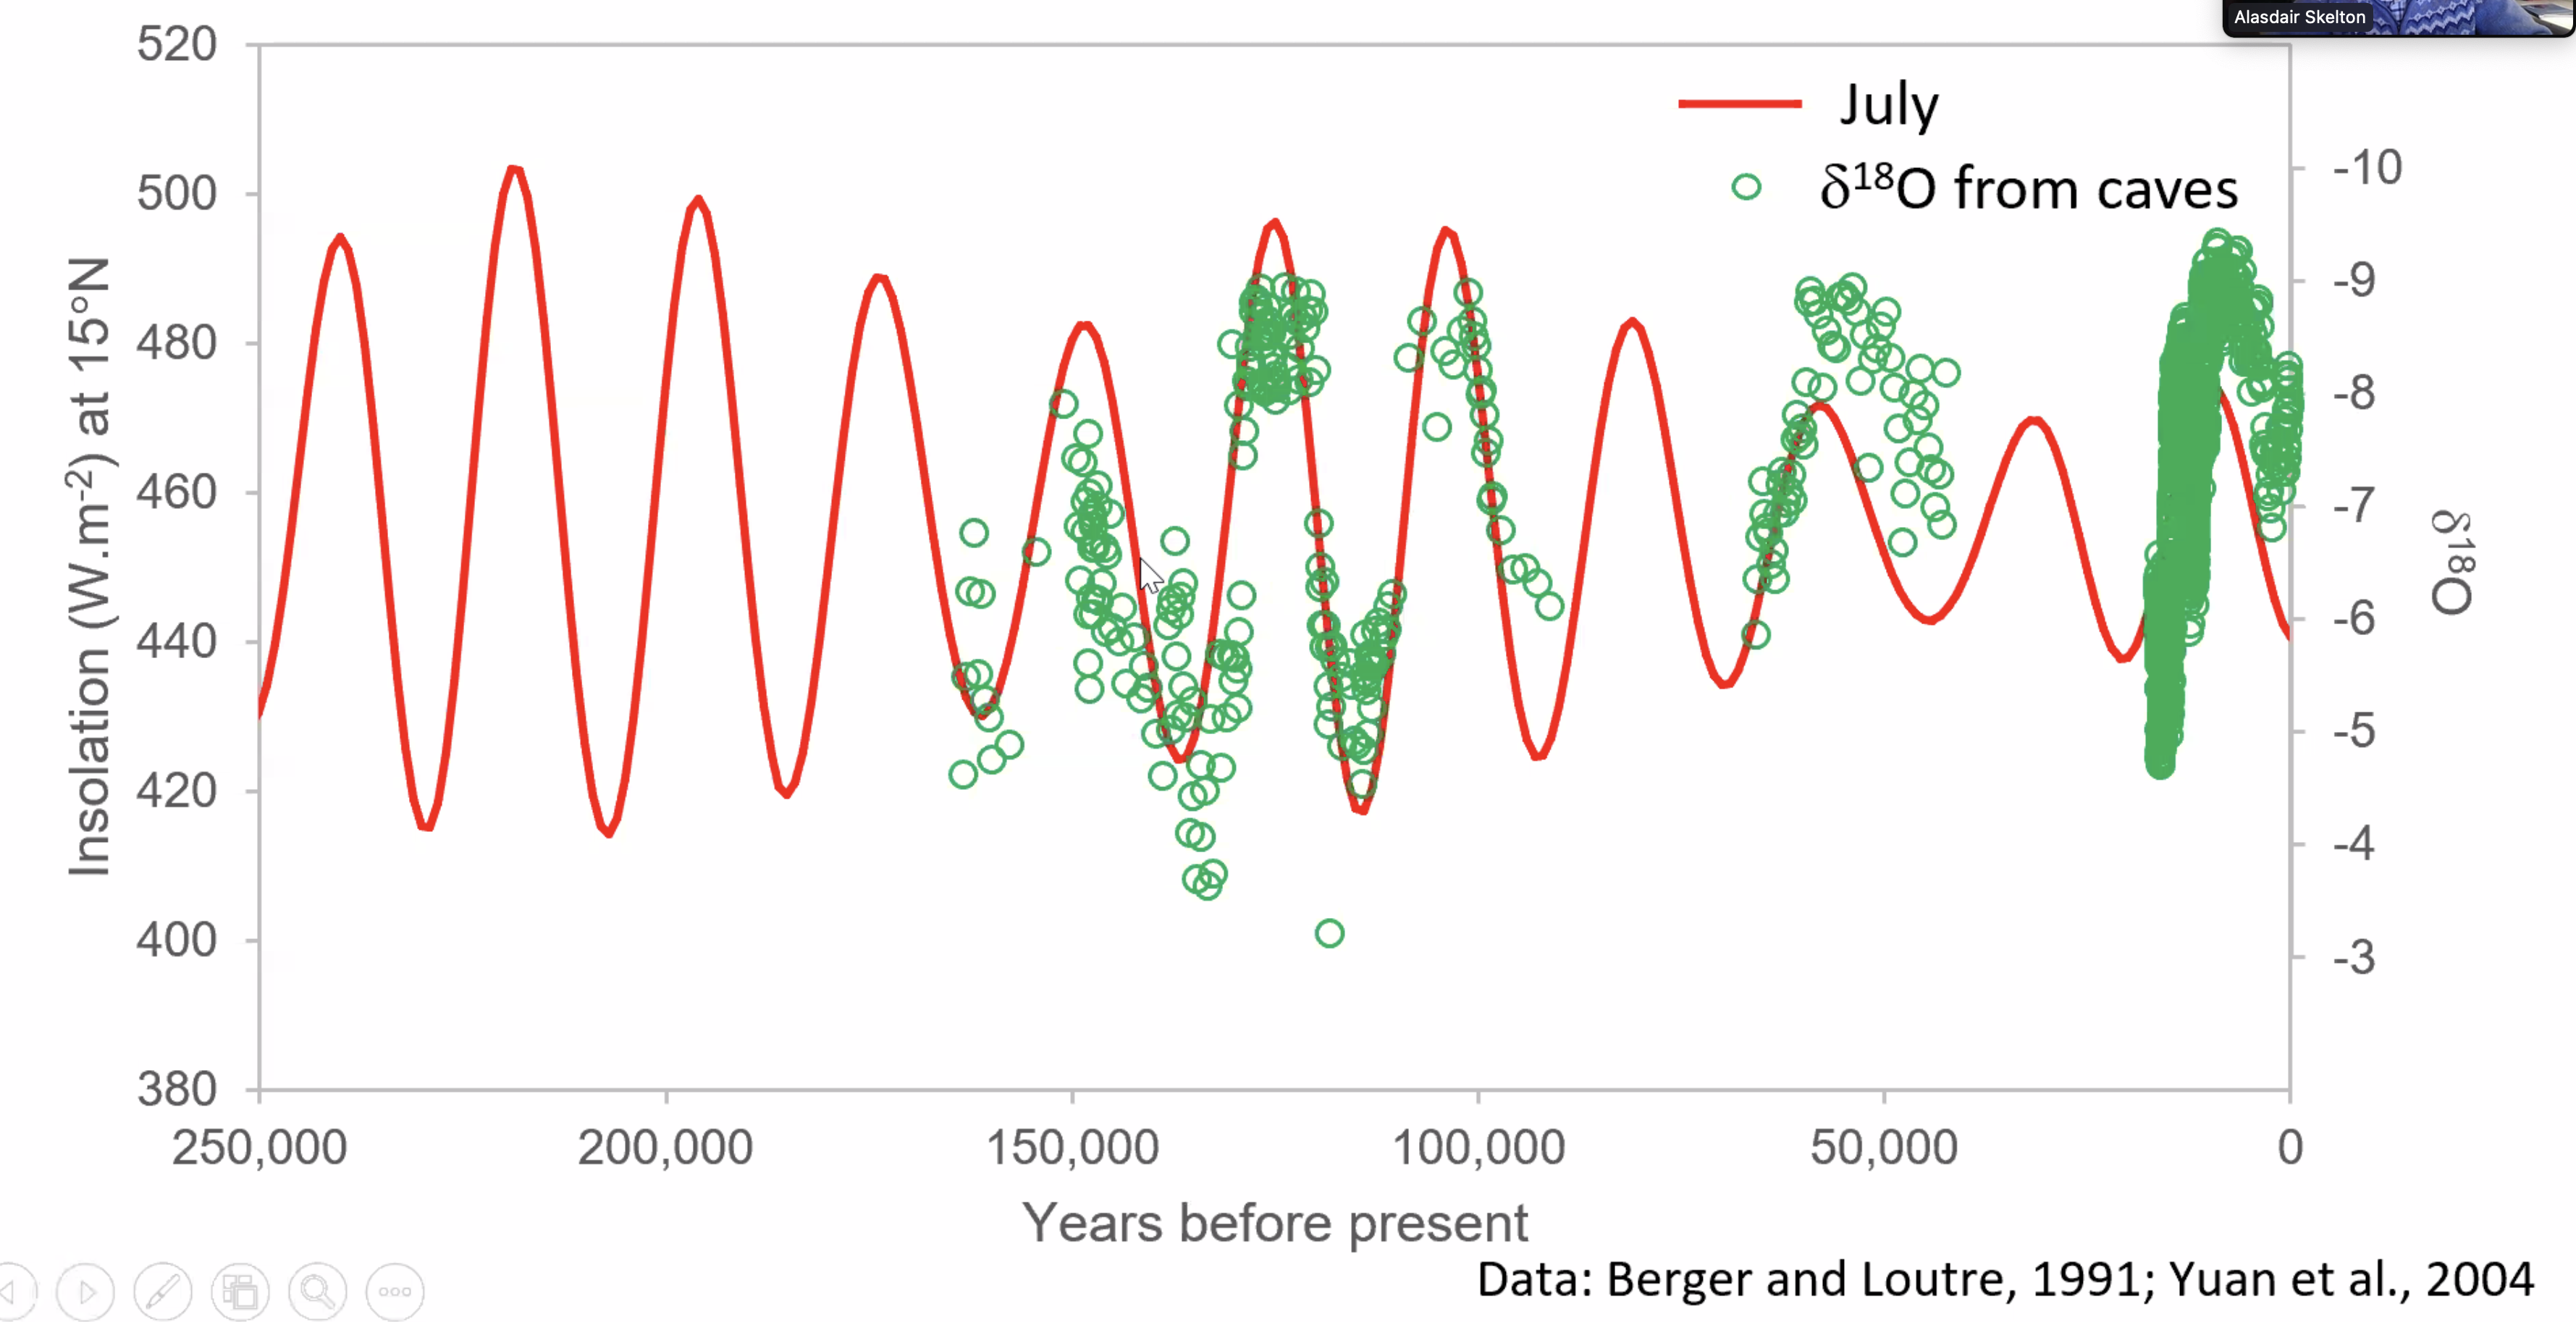
\includegraphics[width=0.75\linewidth]{content/img/monsoons_cave_proxy.png}
\end{figure}

\subsection{Glaciations}

\begin{figure}[H]
    \centering
    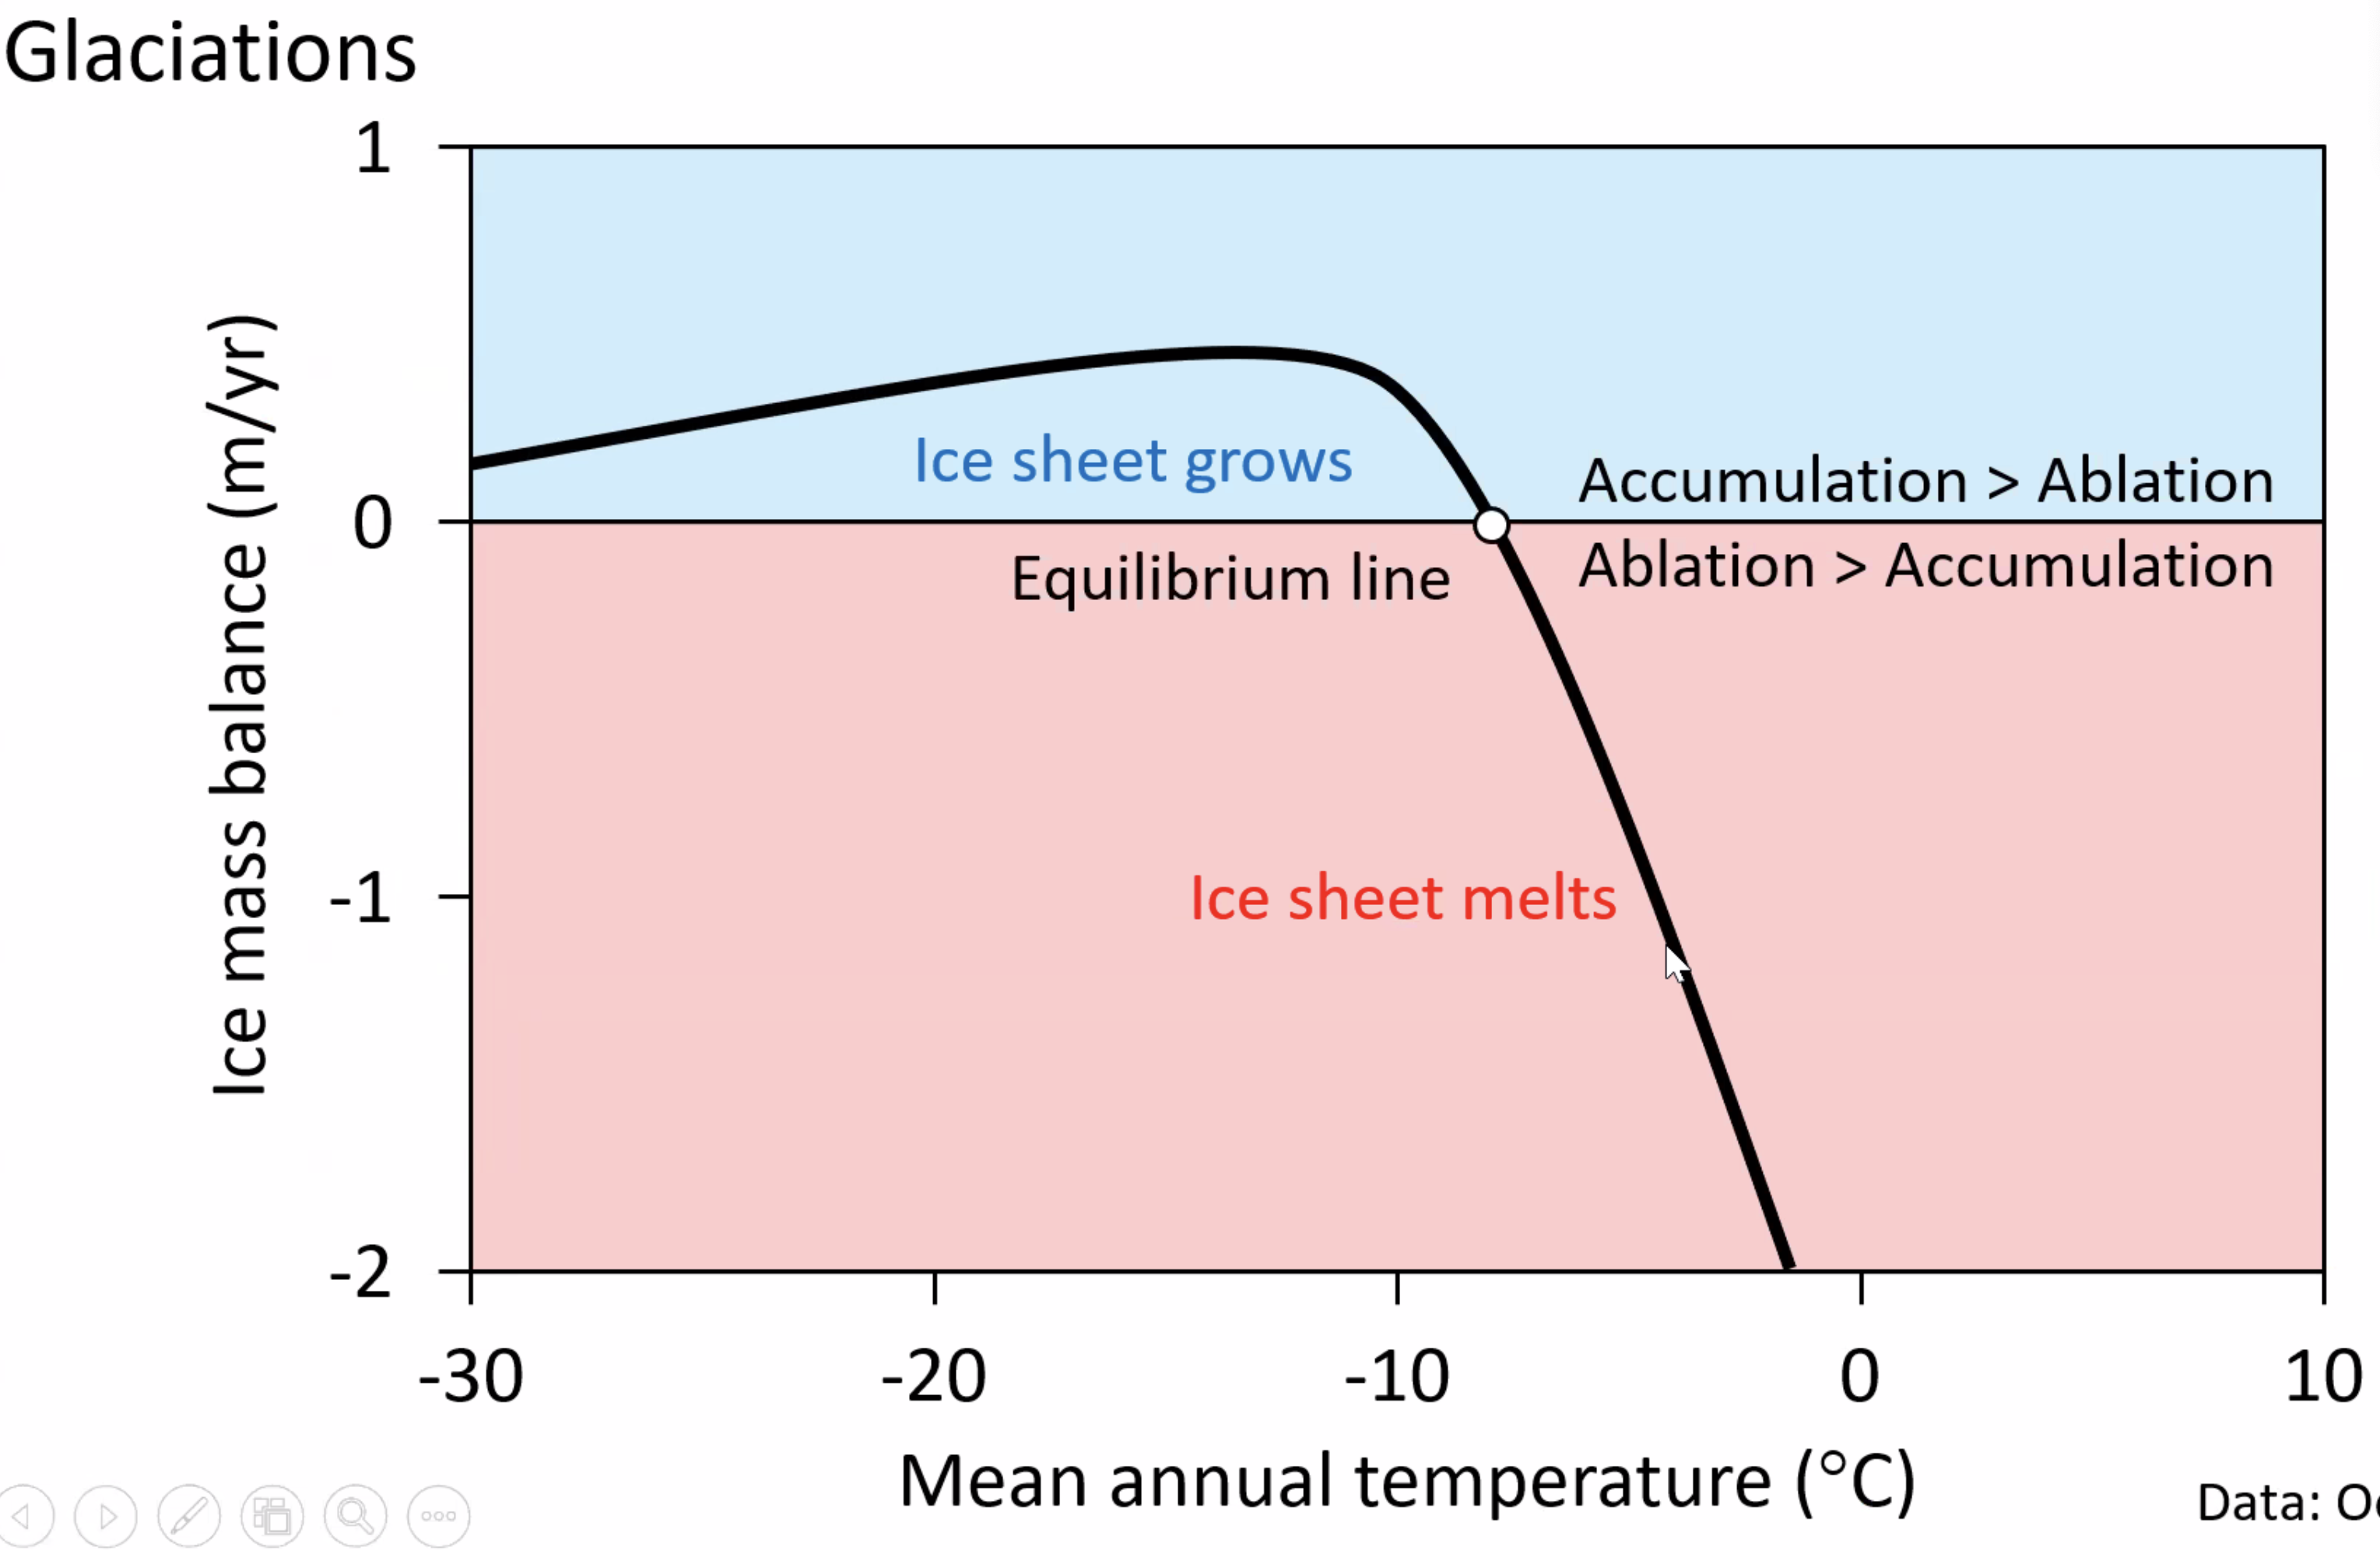
\includegraphics[width=0.75\linewidth]{
    content/img/ice_sheet_equilibrium.png}
\end{figure}

\begin{figure}[H]
    \centering
    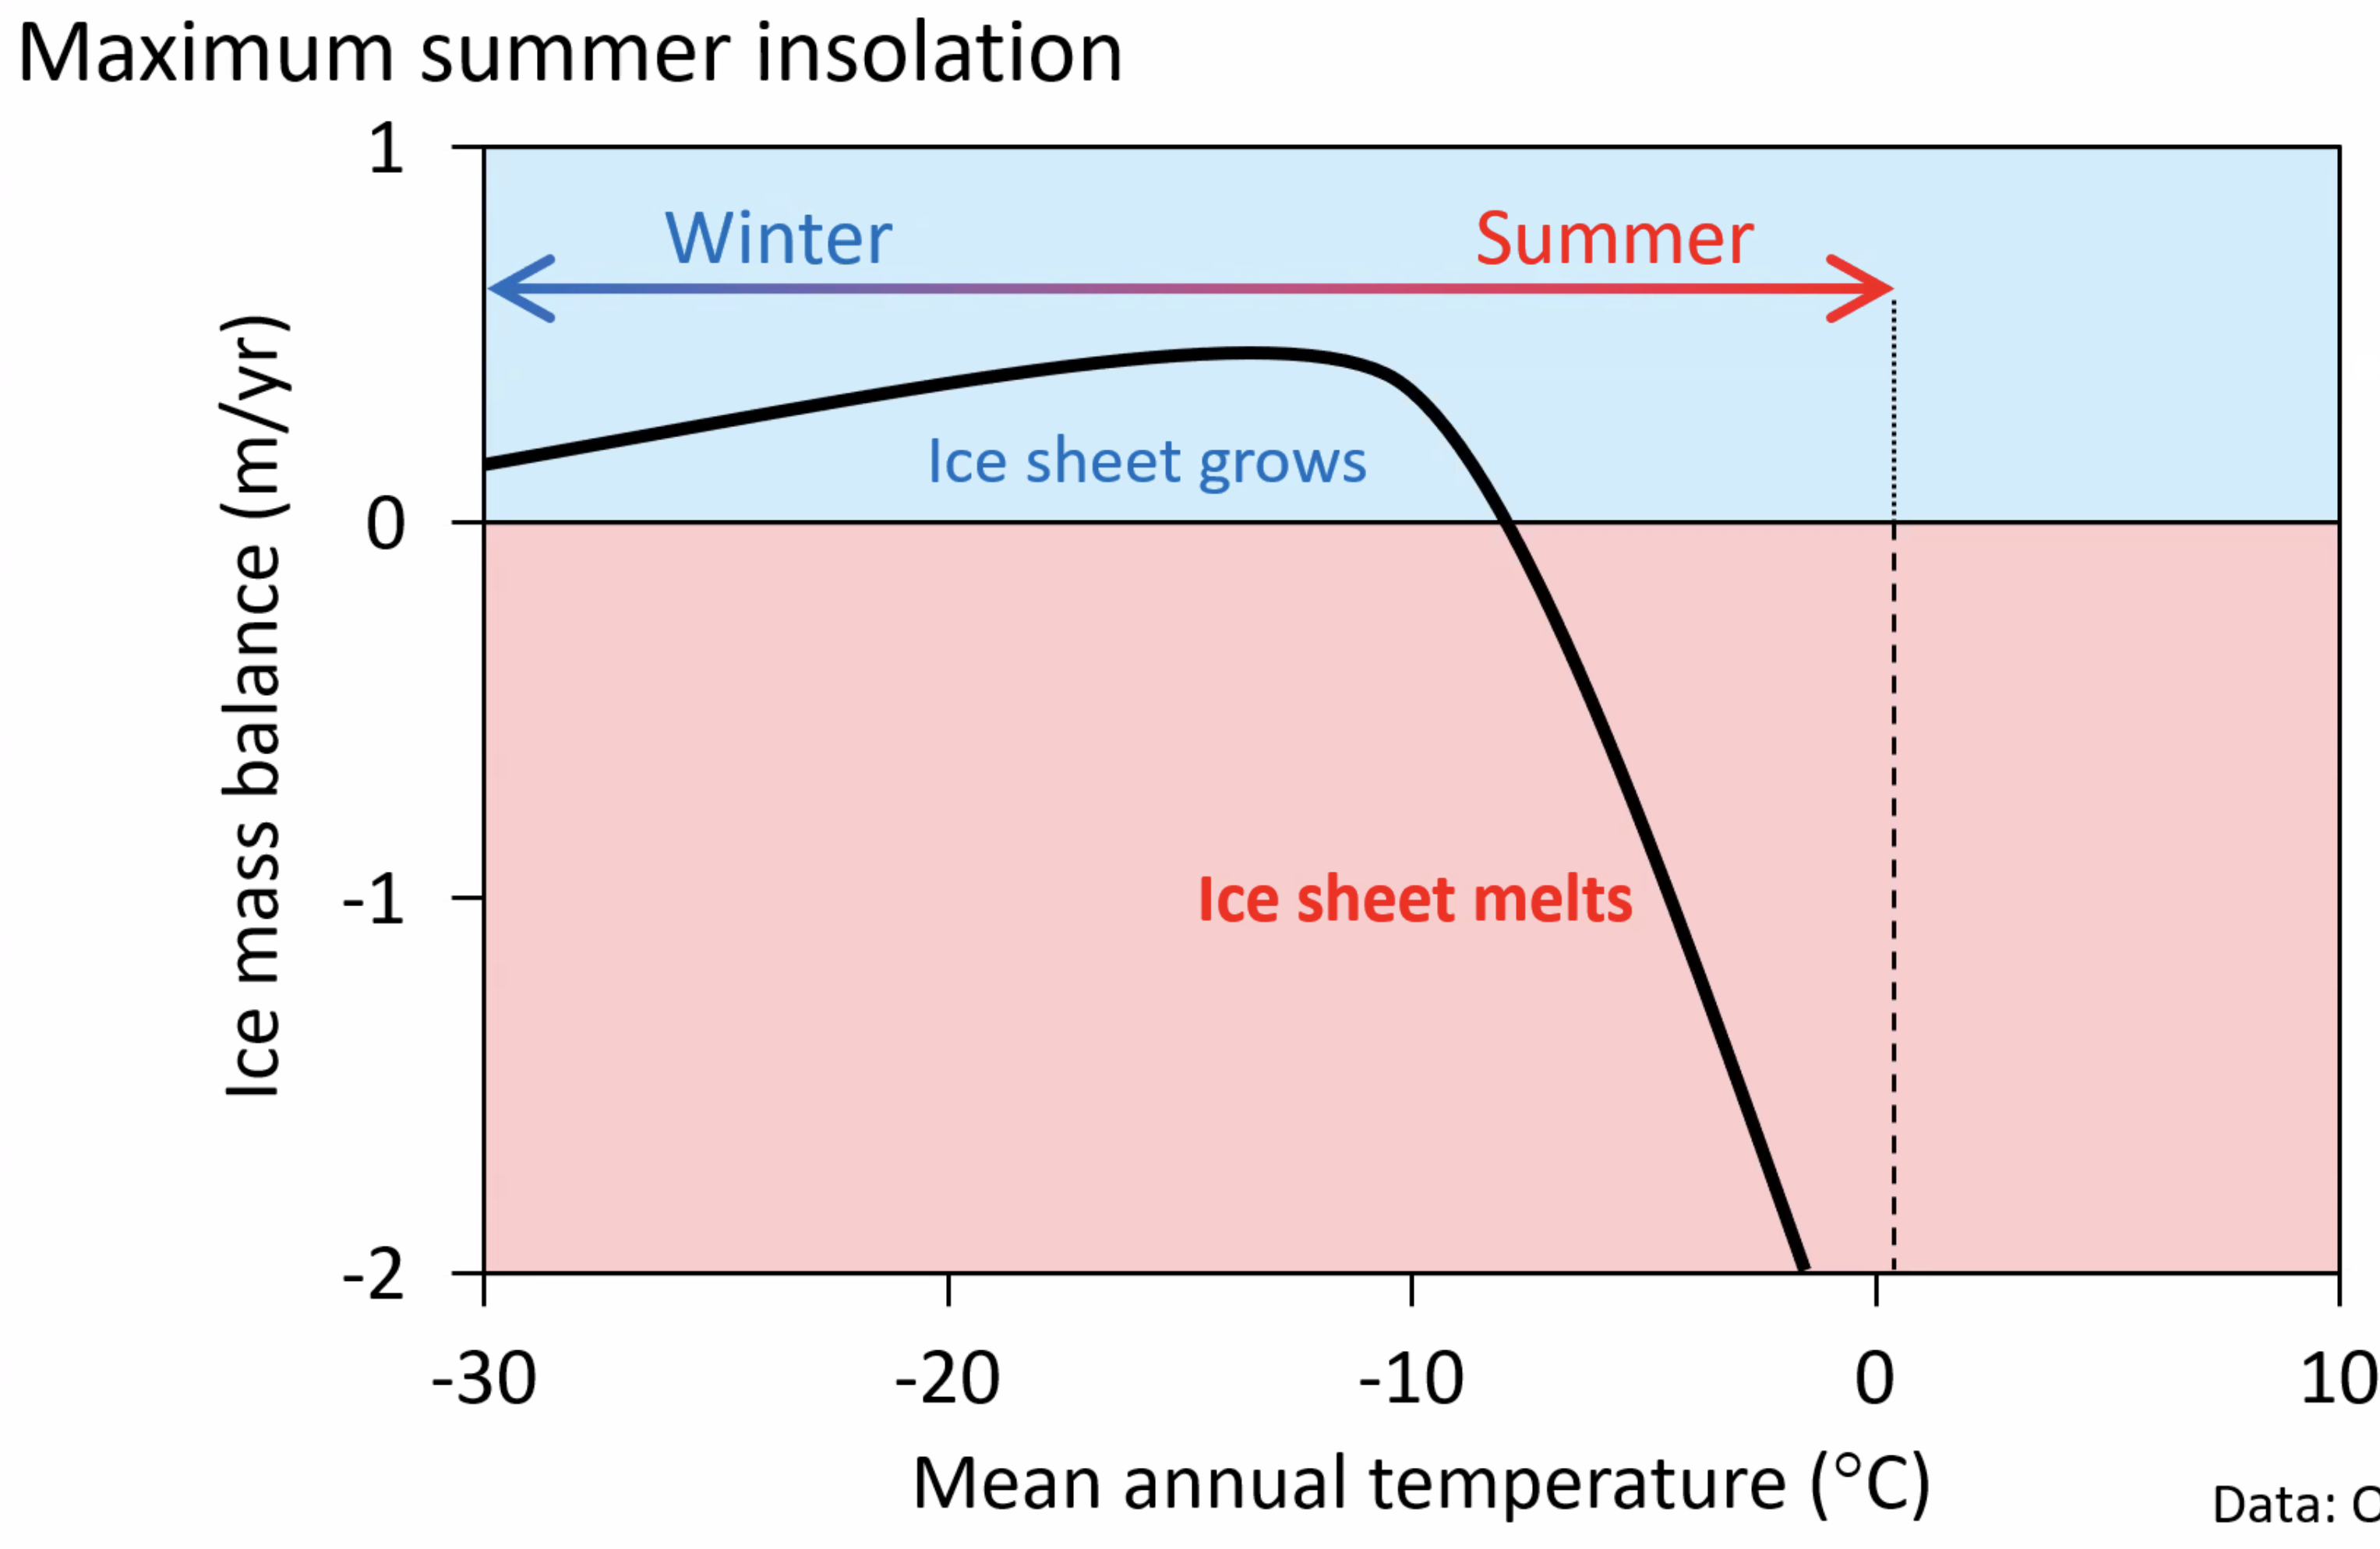
\includegraphics[width=0.75\linewidth]{
    content/img/maximum_summer_insolation.png}
    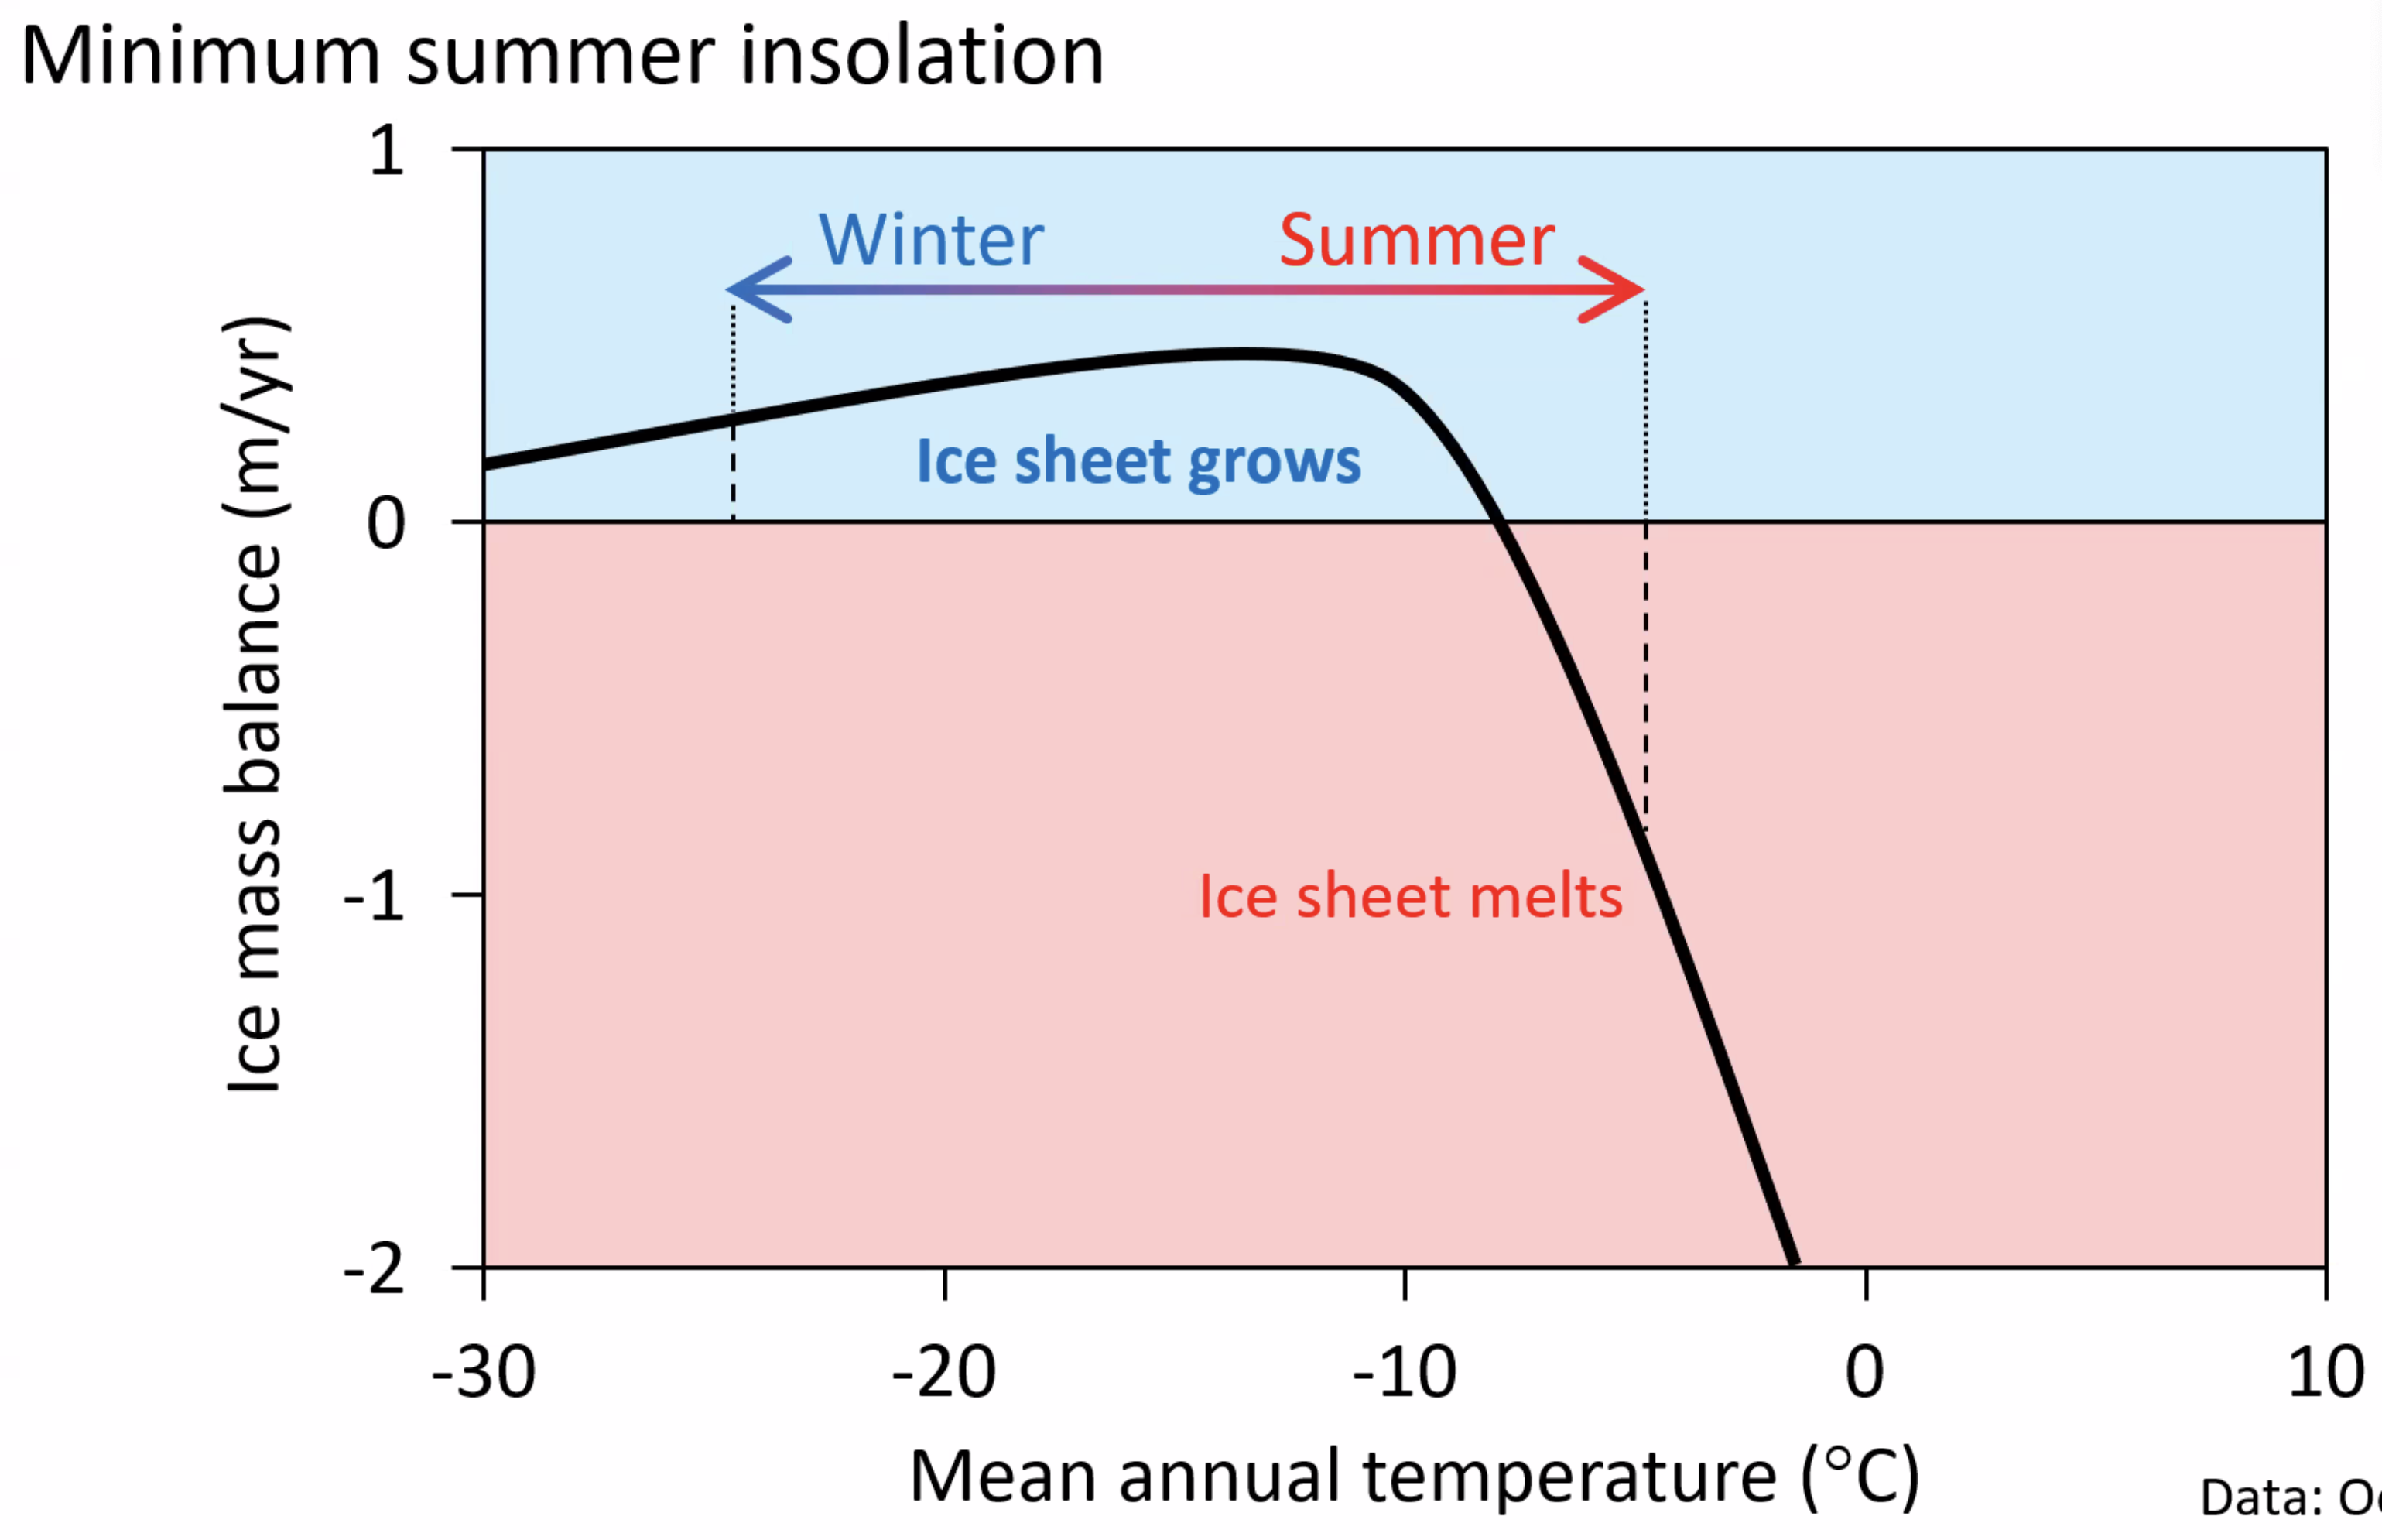
\includegraphics[width=0.75\linewidth]{
    content/img/minimum_summer_insolation.png}
\end{figure}

\begin{figure}[H]
    \centering
    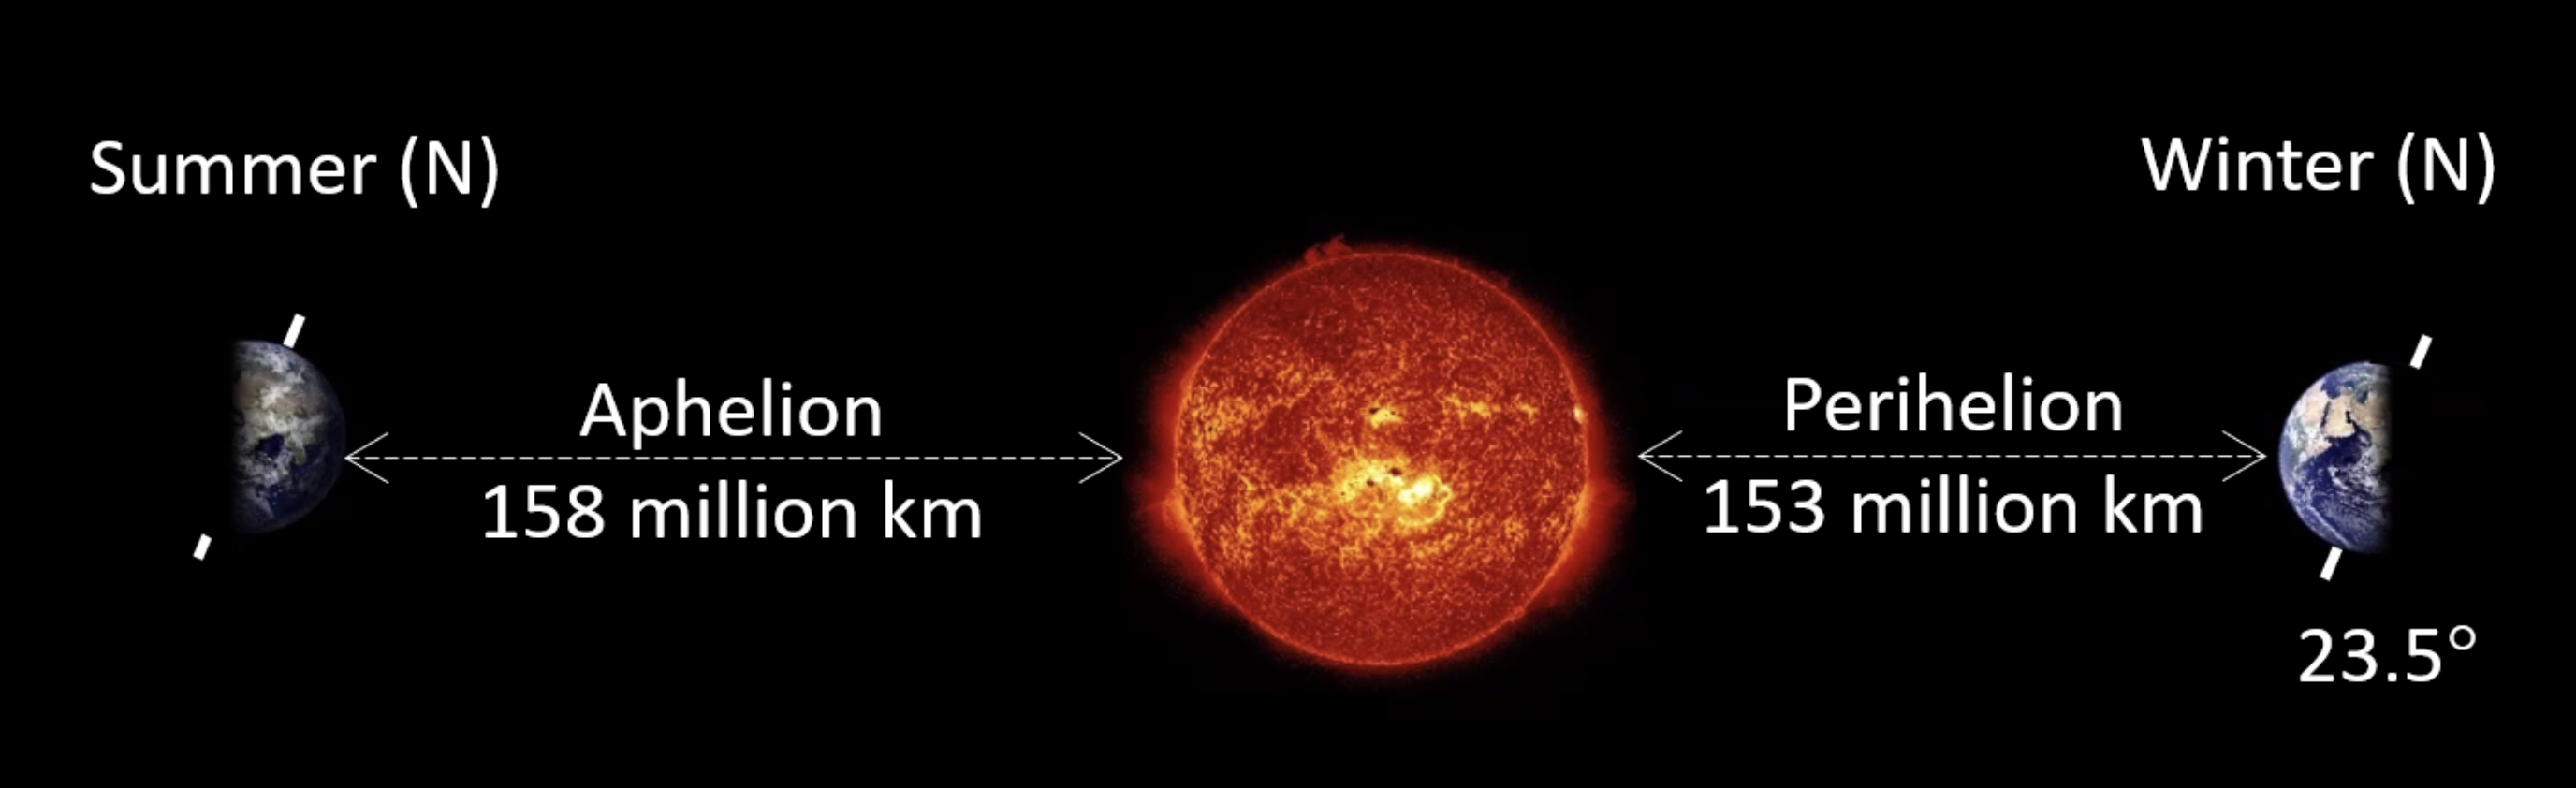
\includegraphics[width=0.75\linewidth]{
    content/img/aphelion_perihelion.png}
    \caption{Currently, axial tilt and eccentricity have opposite effects.
    Tilt is dominating which is why we are currently in interglacial.}
\end{figure}

\begin{figure}[H]
    \centering
    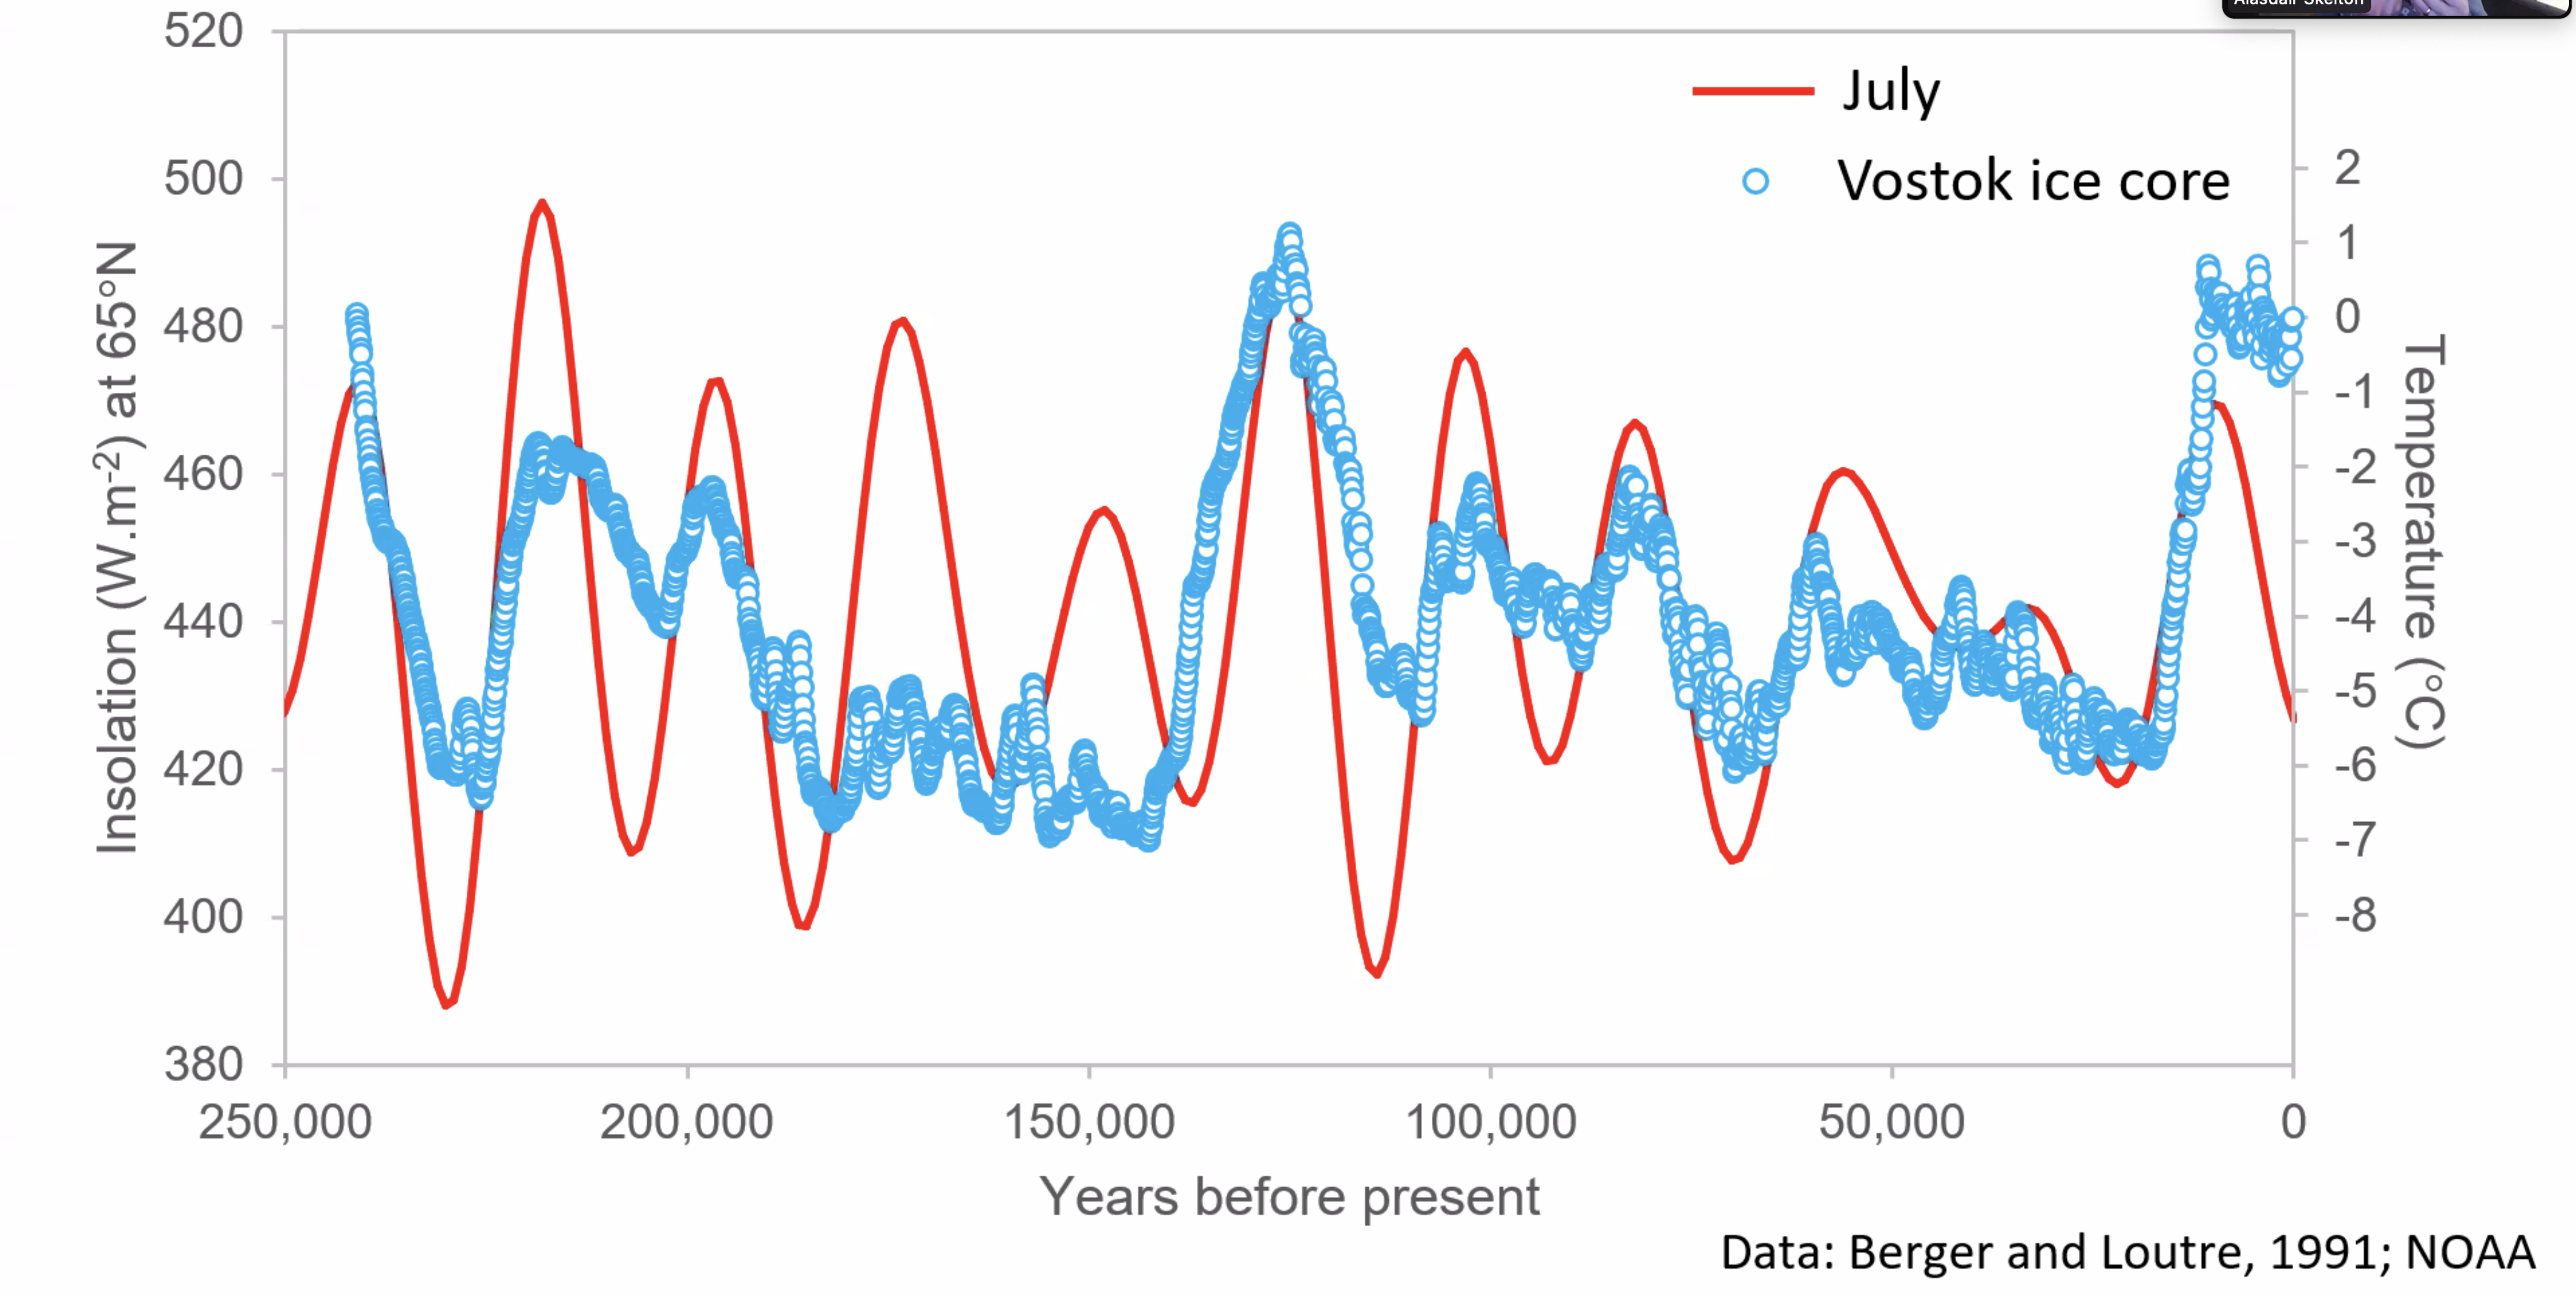
\includegraphics[width=0.75\linewidth]{content//img/vostok_ice_core.png}
\end{figure}
